\documentclass[11pt,a4paper]{article}

\usepackage{amsfonts,amssymb,amsmath}
\usepackage[margin=1in]{geometry}
\usepackage[none]{hyphenat}
\usepackage{graphicx}
\usepackage{fancyhdr}
\usepackage{float}
\usepackage{color}
\usepackage{xcolor}
\usepackage{tikz}
\usepackage{polynom}
\usepackage{bigints}
\usepackage{esint}
\usepackage[nottoc,notlot,notlof]{tocbibind}

\usetikzlibrary{quotes,angles,graphs,patterns,fadings,arrows.meta,shapes,trees,bending}

% grad, div and curl are operator NAMES. Set as bare letters in maths they come
% out italic, so "grad" reads as the product g.r.a.d - the same defect as a bare
% \cos. These give them upright type and the correct spacing.
\DeclareMathOperator{\grad}{grad}
\DeclareMathOperator{\dive}{div}
\DeclareMathOperator{\curl}{curl}

\parindent 0ex
\setlength{\parskip}{0.55\baselineskip}
% Displays carry their own skips; with a non-zero \parskip on top of them,
% consecutive displays drift apart. Tighten them so a derivation reads as one
% argument rather than as a column of disconnected formulae.
\setlength{\abovedisplayskip}{0.5\baselineskip}
\setlength{\belowdisplayskip}{0.5\baselineskip}
\setlength{\abovedisplayshortskip}{0.25\baselineskip}
\setlength{\belowdisplayshortskip}{0.25\baselineskip}

\pagestyle{fancy}
\fancyfoot[C]{\thepage}
\fancyhead{}
\fancyhead[R]{\rightmark}
\renewcommand{\headrulewidth}{0pt}

% Theorem environments. The source declared none: its 125 examples, 91
% solutions, 21 definitions and 30 theorems were set as red bold text with the
% number typed by hand, so LaTeX numbered nothing and inserting an example meant
% renumbering the rest of the subsection.
\usepackage{amsthm}
\theoremstyle{definition}
% One shared counter running section.subsection.n, as in the other courses here.
\newtheorem{thm}{Theorem}[subsection]
\newtheorem{defn}[thm]{Definition}
\newtheorem{exa}[thm]{Example}
\newtheorem{prop}[thm]{Proposition}
\newtheorem{coro}[thm]{Corollary}
\newtheorem{lem}[thm]{Lemma}
\newtheorem{result}[thm]{Result}
\newtheorem{exe}[thm]{Exercise}
\newtheorem*{note}{Note}
\newtheorem*{remark}{Remark}
\newtheorem{problemx}{Problem}[subsection]
\newenvironment{problem}{\begin{problemx}}{\end{problemx}}
\newenvironment{solution}
  {\renewcommand{\qedsymbol}{}\begin{proof}[\textit{Solution}.]}
  {\end{proof}}
\usepackage{enumitem}
% A heading that is legal inside a theorem body, a list or a float, where
% \subsubsection is not. Same weight as \subsubsection* so the two read alike.
\newcommand{\subhead}[1]{%
  \par\medskip\noindent\textbf{#1}\par\nobreak\smallskip}

\begin{document}
% Title page depersonalised for the web, as with every other course here: no
% university, no lecturers, no author, no year. The identity kept below is the
% open-set definition of continuity, which is the whole point of the subject:
% continuity survives when distance is thrown away.
\begin{titlepage}
\thispagestyle{empty}
\begin{center}
\vspace*{3cm}
{\Huge\bfseries Topology}\\[1.2cm]
{\large Lecture Notes}\\[2.5cm]
\line(1,0){300}\\[1.5cm]
$$f \text{ continuous} \iff f^{-1}(V) \text{ open for every open } V$$
\end{center}
\end{titlepage}

\tableofcontents
\thispagestyle{empty}
\clearpage
\setcounter{page}{1}
















\pagebreak
\section*{Introduction}
In previous courses you studied continuity of functions whose domain and range is the set of real numbers. Continuous functions where in this case defined in terms of the absolute value on the set of real numbers.\\ The absolute value is a distance function in the sense that if$ x$ and $y$ are any two real numbers, then $|x-y|$ gives the distance between $x$ and $y$.\\ In this course will introduce a general type of distance function, called a\\ metric, which will enable us to define continuity of functions in a more\\ abstract way.\\ This is desirable because we are then able to discuss continuity of functions defined on various types of sets not only sets of real numbers. We will go a step further and discuss continuity of functions in an even more general settings where the notation of distance is not used to define a continuous function. To achieve this, certain collections of sets called topologies, will play a prominent role.\\ In the light of previous paragraphs, this course is about metric and\\ topological spaces.\\ A metric space is a set $X$ endowed with a metric $d$ while a topological space is a set $X$ together with a collection $\tau$ of subsets of $X$ that forms a topology.\\Metric and topological spaces have applications in various branches of\\ mathematics and its applications.\\












\pagebreak
\section{METRIC SPACES}
\vspace{0.5cm}

\begin{center}
\textbf{Definition and Examples of Metric Spaces}
\end{center}

\begin{defn}
Let X be a non-empty set. A function $d:X\times X\rightarrow \mathbb{R}$ is called a metric if it satisfies the following for all $x,y,z\in X$,
\begin{enumerate}
\item[i] $d(x,y)\geq 0$
\item[ii] $d(x,y)=0$ if and only if $x=y$
\item[iii] $d(x,y)=d(y,x)$
\item[iv] $d(x,z)\leq d(x,y)+d(y,z)$ (triangle inequality)
\end{enumerate}

The pair $(X,d)$ is called a metric space.\\\\














\textbf{Example}\\ The function $d(x,y)=|x-y|$ defines a metric on $\mathbb{R}$. This is called the usual metric on $\mathbb{R}$.\\\\
\end{defn}
\begin{proof}
By definition, the absolute value on $\mathbb{R}$ is non-negative. Therefore\\ $d(x,y)=|x-y|\geq 0$. Now since $|x-y|=0$ if and only if $x=y$. It follows that $d(x,y)=0$ if and only if $x=y$. To verify the third axiom, we have\\
$d(x,y)=|x-y|=|-(x-y)|=|y-x|=d(y,x)$.\\
To verify the triangle inequality. Suppose that $x,y,z\in X$ then\\
$d(x,y)=|x-z|=|x-y+y-z|\leq |x-y|+|y-z|=d(x,y)+d(y,z)$\\\\
Thus, $(\mathbb{R},d)$ is a metric space.\\\\
\end{proof}




\begin{exa}
The modulus function $d(z_1,z_2)=|z_1-z_2|$ defines a metric on $\mathbb{C}$.\\

In order to prove the next example,the following theorem is required.\\
\end{exa}



\begin{thm}[Minkowski's Inequality]
Let $\iota^2$ be the set of all sequences of real numbers satisfying $\sum\limits^{\infty}_{n=1} a^2_n < \infty$. If $x=(x_n), y=(y_n) \in \ell^2$, then $x+y=(x_n+y_n)\in \ell^2$ and
$$\Bigg[\sum\limits^{\infty}_{n=1} (x_n+y_n)\Bigg]^{1/2} \leq \Bigg[\sum\limits_{n=1}^{\infty} x^2_n\Bigg]^{1/2}+\Bigg[\sum\limits_{n=1}^{\infty} y^2_n\Bigg]^{1/2}$$\\\\\\










\textbf{Example}\\ The following functions define metrics on $\mathbb{R}^2$
\begin{enumerate}
\item[i] $d_1(x,y)=|x_1-y_1|+|x_2-y_2|$, where $x=(x_1,x_2), y=(y_1,y_2)\in \mathbb{R}^2$
\item[ii] $d_2(x,y)=\sqrt{(x_1-y_1)^2 +(x_2-y_2)^2}$
\item[iii] $d_3(x,y)=\max\{|x_1-y_1|,|x_2-y_2|\}$\\\\
\end{enumerate}
\end{thm}




\begin{proof}
\begin{enumerate}
\item[i]  Since $d_1$ is the sum of the absolute value function on $\mathbb{R}^2$, it is non-negative and $d_1=|x_1-y_1|+|x_2-y_2| \geq 0$ for all $x,y\in \mathbb{R}^2$.\\ To verify that $d_1(x,y)=0$ if and only if $x=y$, we have that \\$|x_1-y_1|+|x_2-y_2|=0$ if and only if $x_1=y_1$ and $x_2=y_2$. This implies that $d_1(x,y)=0$ if and only if $x=y$.\\ We show that $d_1(x,y)=d_2(y,x)$ for all $x,y\in \mathbb{R}^2$. We have that 
\begin{align*}
d_1(x,y) & =|x_1-y_1|+|x_2-y_2|=|-(y_1-x_1)|+|-(y_2-x_2)|\\
         & =|y_1-x_1|+|y_2-x_2|\\
         & = d_1(y,x)
\end{align*}         
Finally, we prove that the triangle inequality holds.\\ Let $x=(x_1,x_2), y=(y_1,y_2), z=(z_1,z_2)\in \mathbb{R}^2$. Then 
\begin{align*}
d_1(x,z) &=|x_1-z_1|+|x_2-z_2|\\
         &=|x_1-y_1+y_1-z_1|+|x_2-y_2+y_2-z_2|\\
         &\leq |x_1-y_1|+|y_1-z_1|+|x_2-y_2|+|y_2-z_2|\\
         &=(|x_1-y_1|+|x_2-y_2|) +(|y_1-z_1|+|y_2-z_2|)\\
         &=d_1(x,y)+d_1(y,z)
\end{align*}











\pagebreak
\item[ii] For any $x=(x_1,x_2), y=(y_1,y_2)\in \mathbb{R}^2$.\\ we have that $\sqrt{(x_1-y_1)^2+(x_2-y_2)^2}\geq 0$ so that $d_2(x,y)\geq 0$.\\ Also, $(x_1-y_1)^2+(x_2-y_2)^2=0$ if and only if $x_1-y_1=0$ and $x_2-y_2=0$. In other words $(x_1-y_1)^2+(x_2-y_2)^2=0$ if and only if $x_1=y_1$ and $x_2=y_2$. This means that $d_2(x,y)=0$ if and only if $x=y$.\\ To show that $d_2(x,y)=d_2(y,x)$, we just observe that\\ $(x_1-y_1)^2=(-(-x_1+y_1))^2=(y_1-x_1)^2$ and\\ $(x_2-y_2)^2=(-(-x_2+y_2))^2=(y_2-x_2)^2$.This imply that

\begin{align*}
d_2(x,y) &=\sqrt{(x_1-y_1)^2+(x_2-y_2)^2}\\
         &=\sqrt{(y_1-x_1)^2+(y_2-x_2)^2}\\
         &=d_2(y,x)
\end{align*}
To verify the triangle inequality, let $x=(x_1,x_2), (y_1,y_2), (z_1,z_2)\in \mathbb{R}^2$. Then
\begin{align*}
d_2(x,z) &=\sqrt{(x_1-z_1)^2+(x_2-z_2)^2}\\
         &=\sqrt{(x_1-y_1+y_1-z_1)^2+(x_2-y_2+y_2-z_2)^2}\\
         &=\sqrt{(a_1+b_1)^2+(a_2+b_2)^2}
\end{align*}
where $a_1=x_1-y_1$, $b_1=y_1-z_1$, $a_2=x_2-y_2$, $b_2=y_2-z_2$.\\ By applying Minkowski's inequality, we obtain that $$\sqrt{(a_1+b_1)^2+(a_2+b_2)^2}\leq \sqrt{a^2_1 +a_2^2}+\sqrt{b_1^2+b_2^2}$$ Substituting for $a_1,a_2,b_1,b_2$ we obtain that $$d_2(x,z)\leq d_2(x,y)+d_2(y,z).$$\\












\pagebreak
\item[iii] If $x=(x_1,x_2), y=(y_1,y_2) \in \mathbb{R}^2$, we see that $|x_1-y_1|\geq 0$ and $|x_2-y_2|\geq 0$ so that $d_3(x,y)=\max\{|x_1-y_1|,|x_2-y_2|\}\geq 0$.\\ Also, $\max\{|x_1-y_1|,|x_2-y_2|\}=0$ if and only if $|x_1-y_1|=0$ and $|x_2-y_2|=0$, which means that $\max\{|x_1-y_1|,|x_2-y_2|\}=0$ if and only if $x_1=y_1$ and $x_2=y_2$. Thus $d_3=0$ if and only if $x=y$.\\ We show that $d_3(x,y)=d_3(y,x)$. Since $$\max\{|x_1-y_1|,|x_2-y_2|\}=\max\{|y_1-x_1|,|y_2-x_2|\}$$ we have that $d_3(x,y)=d_3(y,x)$.\\ To show the triangle inequality holds, let $x=(x_1,x_2), y=(y_1,y_2),\\ z=(z_1,z_2)\in \mathbb{R}^2$. Then
\begin{align*}
d_3(x,z) &=\max\{|x_1-z_1|,|x_2-z_2|\}\\
         &=\max\{|x_1-y_1+y_1-z_1|,|x_2-y_2+y_2-z_2|\}\\
         &\leq \max\{|x_1-y_1|+|y_1-z_1|,|x_2-y_2|+|y_2-z_2|\}\\
         &\leq \max\{|x_1-y_1|,|x_2-y_2|\} +\max\{|y_1-z_1|,|y_2-z_2|\}\\
         &=d_3(x,y) +d_3(y,z).
\end{align*}            
\end{enumerate}
\end{proof}







\begin{exa}
The function $d(x,y)=\sum\limits_{n=1}^{\infty} |x_n-y_n|$ defines a metric on the set $\ell$ of sequences of real numbers with the property $\sum\limits^{\infty}_{n=1} |x_n| <\infty$.\\
\end{exa}


\begin{proof}
Let $x=(x_n),y=(y_n)\in \ell$. Since $|x_n-y_n|\geq 0$ for all $n\in \mathbb{N}$, we obtain that $d(x,y)=\sum\limits^{\infty}_{n=1} |x_n-y_n|\geq 0$. Also since $|x_n-y_n|=0$ if and only if $x_n=y_n$, it follows that $d(x,y)=0$ if and only if $x=y$.\\ 
From $|x_n-y_n|=|-(-x_n+y_n)|=|y_n-x_n|$, we get that $d(x,y)=d(y,x)$.\\ 
To verify the triangle inequality, let $x=(x_n), y=(y_n), z=(z_n)\in \ell$. From properties of the absolute value on the set of real numbers, we have that
\begin{align*}
\sum^n_{k=1} |x_k-z_k| &=\sum_{k=1}^n |x_k-y_k+y_k-z_k|\\
                       &\leq \sum^n_{k=1} |x_k-y_k| +\sum^n_{k=1} |y_k-z_k|
\end{align*} 
Taking limits on both sides as $n\rightarrow \infty$, we obtain that\\ $\sum\limits^{\infty}_{k=1} |x_k-z_k|\leq \sum\limits_{k=1}^{\infty} |x_k-y_k|+\sum\limits^{\infty}_{k=1} |y_k-z_k|.$\hspace{0.2cm} Hence $d(x,z)\leq d(x,y)+d(y,z)$.\\\\
\end{proof}








\begin{exa}
The function $d(x,y)=\sum\limits^{\infty}_{n=1} \dfrac{1}{2^n}\,\dfrac{|x_n-y_n|}{1+|x_n-y_n|}$ defines a metric on the set $\mathbb{R}^{\mathbb{N}}$ of sequences of real numbers.\\
\end{exa}



\begin{proof}
Let $x=(x_n), y=(y_n)\in \mathbb{R}^{\mathbb{N}}$. Using the properties of the absolute value on the set of real numbers, the properties $d(x,y)\geq 0$, $d(x,y)=0$ if and only if $x=y$ and $d(x,y)=d(y,x)$ are easily established.\\ Let $x=(x_n), y=(y_n), z=(z_n)\in \mathbb{R}^{\mathbb{N}}$. To verify that the triangle inequality holds we prove the inequality $\dfrac{|a+b|}{1+|a+b|}\leq \dfrac{|a|}{1+|a|}+\dfrac{|b|}{1+|b|}$\\ From the fact that $\dfrac{1}{|a|+|b|}<\dfrac{1}{|a+b|}$, it follows that\\
\begin{align*}
\frac{|a+b|}{1+|a+b|} &=\frac{1}{1+\dfrac{1}{|a+b|}}\\
                      &\leq \frac{1}{1+\dfrac{1}{|a|+|b|}}=\frac{|a|+|b|}{1+|a|+|b|}\\\\
                      &=\frac{|a|}{1+|a|+|b|}+\frac{|b|}{1+|a|+|b|}\\\\
                      &\leq \frac{|a|}{1+|a|}+\frac{|b|}{1+|b|}
\end{align*}
Therefore, $\dfrac{|a+b|}{1+|a+b|}\leq \dfrac{|a|}{1+|a|}+\dfrac{b}{1+b}$, if we take $a=x_n-y_n$ and\\ $b=y_n-z_n$ in this inequality, we obtain that
$$\frac{|x_n-z_n|}{1+|x_n-z_n|}\leq \frac{|x_n-y_n|}{1+|x_n-y_n|}+\frac{|y_n-z_n|}{1+|y_n-z_n|}$$
from which it follows that $d(x,z)\leq d(x,y)+d(y,z)$.\\\\

Note that alternatively, one can use the fact that $f(x)=\dfrac{x}{1+x}$ is a \\monotone increasing function to prove the last example.\\\\\\ 
\end{proof}













\begin{exa}
If X is any non-empty set, the map $d:X\times X\rightarrow \mathbb{R}$ given by\\
\[ d(x,y)=
\begin{cases}
1 & \text{if}\hspace{0.2cm} x\neq y\\
0 & \text{if}\hspace{0.2cm} x=y
\end{cases}
\]
defines a metric on X. This is called the discrete metric on X.\\
\end{exa}

\begin{proof}
By definition $d(x,y)\geq 0$, $d(x,y)=0$, if and only if $x=y$ and\\ $d(x,y)=d(y,x)$ for all $x,y\in X$.\\ To show that the triangle inequality holds, let $x, y,z\in X$. if $x=z$, then $d(x,z)=0$ and $d(x,z)\leq d(x,y)+d(y,z)$ holds. Suppose that $x\neq z$. If $y=z$, then $x\neq y$, so that $d(x,z)=1$, $d(x,y)=1$ and $d(y,z)=0$. Thus $d(x,z)\leq d(x,y)+d(y,z)$. If $y\neq z$ then $d(x,z)=1$, $d(y,z)=1$, which imply that $d(x,z)\leq d(x,y)+d(y,z)$.\\\\\\
\end{proof}












\subsection{Open Sets, Neighbourhoods and Interior Points}
In this section we will discuss subsets of metric spaces that play an important role in further development of several aspects of the theory of metric spaces.\\



\begin{defn}
Let (X,d) be a metric space, $x_0$ a point in X and $r>0$ a real number. Then
\begin{enumerate}
\item[i] the open ball of radius r centered at $x_0$ is the set $$B(x_0,r)=\{x\in X:d(x,x_0)<r\}$$
\item[ii] the closed ball of radius r and centered at $x_0$ is the set $$B[x_0,r]=\{x\in X:d(x,x_0)\leq r\}$$
\item[iii] the sphere of radius r centered at $x_0$ is the set $$S(x_0,r)=\{x\in X:d(x,x_0)=r\}$$\\
\end{enumerate}


\textbf{Note:}\hspace{0.3cm} $S(x_0,r)=B[x_0,r]-B(x_0,r)$\\\\
\end{defn}





\begin{exa}
Consider the metric space $(\mathbb{R},d)$ where d is the usual metric on $\mathbb{R}$. Then every open interval is an open ball and every closed interval is a closed ball. Moreover, any two distinct points $a,b\in \mathbb{R}$ determine a sphere.\\
\end{exa}

\begin{proof}
If we take $x_0=\dfrac{a+b}{2}$ and $r=\dfrac{|a-b|}{2}$, then the open ball interval (a,b) is the open ball $B(x_0,r)$ and the closed interval $[a,b]$ is the closed ball $B[x_0,r]$. \\ Furthermore, if a and b are distinct real numbers, we obtain the sphere $S(x_0,r)=\{x\in \mathbb{R}:|x-y|=r\}=\{a,b\}$.\\\\\\
\end{proof}

\begin{exa}
Consider $\mathbb{R}^2$, with the metrics, $d_1(x,y)=|x_1-y_1|+|x_2-y_2|$,\\ $d_2(x,y)=\sqrt{(x_1-y_1)^2+(x_2-y_2)^2}$ and $d_3(x,y)=\max\{|x_1-y_1|,|x_2-y_2|\}$. Find the open ball of radius 1 centered at (0,0) with respect (i) $d_1$, (ii) $d_2$, (iii) $d_3$.\\
\end{exa}

\begin{solution}
\begin{enumerate}
\item[i]
\begin{align*} 
B((0,0),1) &=\{(x_1,x_2)\in \mathbb{R}^2:d_1((0,0),(x_1,x_2))<1\}\\
           &=\{(x_1,x_2)\in \mathbb{R}^2:|x_1|+|x_2|<1\}
\end{align*}
% you need to draw the diagram    
\begin{figure}[H]
\centering
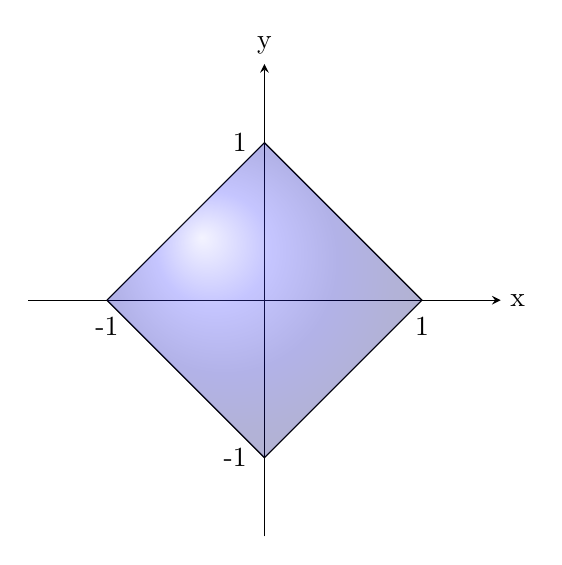
\begin{tikzpicture}[>=stealth]
\draw[->](-3,0)--(3,0)node[right]{\text{x}};
\draw[->](0,-3)--(0,3)node[above]{\text{y}};
\draw(-2,0)--(0,2)--(2,0)--(0,-2)--(-2,0);
\draw[ball color=blue,opacity=0.3](-2,0)--(0,2)--(2,0)--(0,-2)--(-2,0);
\draw(-2,-0.1)node[below]{-1}
(2,-0.1)node[below]{1}
(-0.1,2)node[left]{1}
(-0.1,-2)node[left]{-1};
\end{tikzpicture}
\end{figure}















This set represents the interior of the region bounded by the lines $x_1+x_2=1$, $x_1-x_2=1$, $-x_1+x_2=1$ and $-x_1-x_2=1$\\

\item[ii]
\begin{align*}
B((0,0),1) &=\{(x_1,x_2)\in \mathbb{R}^2:d_2((x_1,x_2),(0,0))<1\}\\
           &=\{(x_1,x_2)\in \mathbb{R}^2:\sqrt{x_1^2+x^2_2}<1\}
\end{align*}
This represents the interior of the circle of radius 1 centered at the origin.\\
%You need to draw the diagram

\begin{figure}[H]
\centering
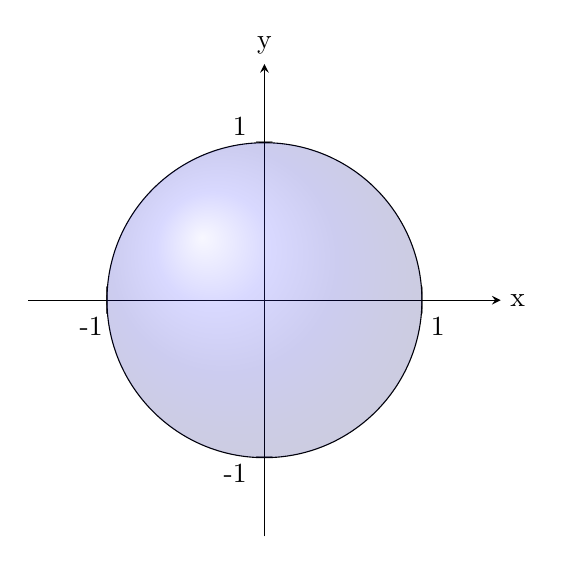
\begin{tikzpicture}[>=stealth]
\draw[->](-3,0)--(3,0)node[right]{\text{x}};
\draw[->](0,-3)--(0,3)node[above]{\text{y}};
\draw(0,0)circle[radius=2cm];
\draw(-2,0)node[]{$|$}
(2,0)node[]{$|$}
(0,-2)node[]{$-$}
(0,2)node[]{$-$};
\shade[ball color = blue, opacity = 0.2] (0,0) circle [radius = 2cm];
\draw(-2.2,-0.1)node[below]{-1}
(2.2,-0.1)node[below]{1}
(-0.1,2.2)node[left]{1}
(-0.1,-2.2)node[left]{-1};
\end{tikzpicture}
\end{figure}














\item[iii] 
\begin{align*}
B((0,0),1) &=\{(x_1,x_2)\in \mathbb{R}^2:d_3((x_1,x_2),(0,0))<1\}\\
           &=\{(x_1,x_2)\in \mathbb{R}^2:\max\{|x_1|,|x_2|<1\}\}
\end{align*}
This represents the interior of the square of diameter 2 centered at the origin.
% A doted diagram





\begin{figure}[H]
\centering
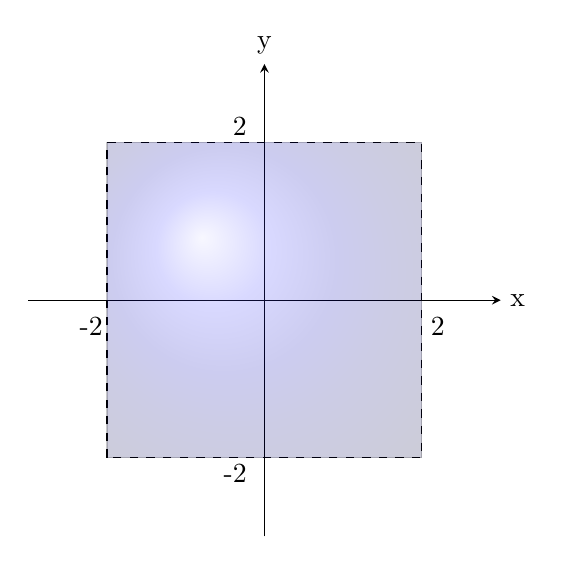
\begin{tikzpicture}[>=stealth]
\draw[->](-3,0)--(3,0)node[right]{\text{x}};
\draw[->](0,-3)--(0,3)node[above]{\text{y}};
\draw[dashed](-2,-2)--(-2,2)--(2,2)--(2,-2)--(-2,-2);
\draw[ball color = blue, opacity=0.2](-2,-2)--(-2,2)--(2,2)--(2,-2)--(-2,-2);
\draw(-2.2,-0.1)node[below]{-2}
(2.2,-0.1)node[below]{2}
(-0.1,2.2)node[left]{2}
(-0.1,-2.2)node[left]{-2};
\end{tikzpicture}
\end{figure}





















\end{enumerate}
\end{solution}

\begin{defn}
Let (X,d) be a metric space. A subset O of X is said to be an open set in X if for every $x\in O$, there is a real number $r>0$ such that $B(x,r)\subseteq O$.\\\\
\end{defn}

\begin{exa}
In the metric space $(\mathbb{R},d)$ where d is usual metric on $\mathbb{R}$, all unions of open intervals are open sets.\\
\end{exa}

\begin{proof}
Let $x\in A$, where A is a union of open intervals in $\mathbb{R}$. Then X belongs to atleast one open intervals. Since every open interval in $\mathbb{R}$ is an open ball, it follows that A is an open set.\\\\
\end{proof}

\begin{thm}
If (X,d) is a metric space, then the union of any collection of open sets in X is open and the intersection of any finite collection of open sets in X is open.\\
\end{thm}

\begin{proof}
Let $\{O_{\lambda}:\lambda \in \Omega\}$ be any family of open sets in X and let $x\in O=\bigcup_{\lambda \in \Omega} O_{\lambda}$. Then $x\in O_{\lambda}$, for at least one $\lambda \in \Omega$. Since $O_{\lambda}$ is open in X, there is an open ball B(x,r) such that $B(x,r)\subseteq O_{\lambda}$. Since $O_{\lambda} \subseteq O$, it follows that $B(x,r)\subseteq O$. Since x was an arbitrary element of O, we obtain that O is an open set in X.\\
To prove the second part, suppose that $O_1,O_2,...........,O_n$ is a finite\\ collection of open sets in X and $O=\bigcap_{k=1}^{n} O_k$. If $x\in O$, then $x\in O_k$ for all $k=1,2,...........n$. Since each $O_k$ is an open set in X, there is an open ball $B(x,r_k)$ such that $B(x,r_k)\subseteq O_k$ for all $k=1,2,.........,n$. Let\\ $r=\min\{r_1, r_2,............,r_n\}$. Then $B(x,r)\subseteq B(x,r_k)$ for all $k=1,2,.........,n$. It follows that $B(x,r)\subseteq O_k$ for all $k=1,2,..........,n$, so that $B(x,r)\subseteq O$. Hence O is open in X.\\\\
\end{proof}

\begin{prop}
If $(X,d)$ is a metric space, then the sets $\emptyset$ and X are both open in X.\\
\end{prop}

\begin{proof}
To show that $\emptyset$ is an open set in X, we need to show that every point in $\emptyset$ is contained in an open ball which is a subset of $\emptyset$. But this holds vacuously since $\emptyset$ has no elements.\\ To prove the second part, if $x\in X$, then every open ball $B(x,r)$ is a subset of X. Hence X is an open set.\\\\
\end{proof}

\begin{defn}
Let $(X,d)$ be a metric space and $x_0\in X$. A subset N of X is said to be a\\ neighbourhood of $x_0$ if there is an open ball $B(x_0,r)$ in X such that\\ $B(x_0,r)\subseteq N$.\\\\
\end{defn}

\begin{prop}
If $(X,d)$ is a metric space, then a subset $O$ of $X$ is open in $X$ if and only if $O$ is a neighbourhood of each of its points.\\
\end{prop}

\begin{proof}
Suppose that $O$ is an open set in $X$ and $x_0\in O$. Then there is a real number $r>0$ such that $B(x_0,r)\subseteq O$, so that $O$ is a neighbourhood of $x_0$. Since $x_0$ was an arbitrary point in $O$, we have that $O$ is a neighbourhood of each of its points.\\ Conversely, suppose that $O$ is a neighbourhood of each of its points. If $x_0\in O$, then there is a real number $r>0$ such that $B(x_0,r)\subseteq O$. Since $x_0$ was an arbitrary point in $O$, it follows that $O$ is open in X.\\\\
\end{proof}

\begin{thm}
Suppose that $(X,d)$ is a metric space and $x_0\in X$. Then the union of any collection of neighbourhoods of $x_0$ is also a neighbourhood of $x_0$ and the intersection of any finite collection of neighbourhoods of $x_0$ is also a neighbourhood of $x_0$.\\
\end{thm}

\begin{proof}
Let $\{N_{\lambda}:\lambda \in \Omega \}$ be a collection of neighbourhoods of $x_0$ and let\\ $N=\bigcup_{\lambda \in \Omega} N_{\lambda}$. Since $N_{\lambda}$ is a neighbourhood of $x_0$ for each $\lambda \in \Omega$, then for each $\lambda$, there exists an open ball $B(x_0,r)$ in X such that $$x_0\in B(x_0,r_{\lambda})\subseteq N_{\lambda}\subseteq \bigcup_{\lambda \in \Omega} N_{\lambda}=N$$ This means that $N$ is a neighbourhood of $x_0$.\\
To prove the second part, suppose that $N_1,N_2,.......,N_n$ is a finite collection of neighbourhoods of $x_0$ and $N=\bigcap^{n}_{k=1} N_k$. Then there exists open balls $B(x_0,r_1), B(x_0,r_2),.......,B(x_0,r_n)$ such that $B(x_0,r_k)\subseteq N_k$ for $k=1,2,......,n$. Let $r=\min\{r_1, r_2,.....,r_n\}$. Then $B(x_0,r)\subseteq B(x_0,r_k)$ for $k=1,2,.....,n$, so that $x_0\in B(x_0,r)\subseteq \bigcap^n_{k=1} N_k =N$. Hence N is a neighbourhood of $x_0$.\\\\
\end{proof}





\begin{defn}
Let (X,d) be a metric space and A a subset of X. A point $x_0$ in X is said to be an interior point of A if A is a neighbourhood of $x_0$. The set of all interior points of A, denoted by Int(A), is called the interior of A.\\\\
\end{defn}

\begin{exa}
Consider the metric space $(\mathbb{R},d)$, where $d$ is the usual metric on $\mathbb{R}$. If $A=[0,1)$ in $\mathbb{R}$, then $Int(A)=(0,1)$.\\
\end{exa}

\begin{proof}
Let $a\in [0,1)$. If $a=0$, then there is no $r>0$ such that $B(a,r)\subseteq [0,1)$. Thus $a\not\in Int(A)$. Suppose that $a\neq 0$. Take $r=\min\{\frac{a}{2},\frac{1-a}{2}\}$. Then $B(a,r)\subseteq [0,1)$ and so $a\in Int(A)$. Hence $Int(A)=(0,1)$.\\\\\\
\end{proof}

\begin{prop}
If $(X,d)$ is a metric space and $A$ a subset of $X$, then $Int(A)$ is the largest open set contained in $A$.\\
\end{prop}

\begin{proof}
We prove that every open set contained in $A$ is contained in $Int(A)$. To this end suppose that $O$ is an open set contained in $A$. Then $O$ is a neighbourhood of each of its points and since $O\subseteq A$, we have that $A$ is a neighbourhood of each of the points of $O$. This implies that $O\subseteq Int(A)$.\\\\
\end{proof}

\begin{defn}
Let $(X,d)$ be a metric space and $A$ a subset of $X$. A point $x_0$ in $A$ is said to be a boundary point of $A$ if every open ball centered at $x_0$ contains points of both $A$ and $A^c$. The set of all boundary points of $A$ is denoted by $bd(A)$ and is called the boundary of $A$.\\\\
\end{defn}

\begin{exa}
Consider the metric space $(\mathbb{R},d)$ where $d$ is the usual metric. Given the set $A=(0,1]$, find $bd(A)$.\\
\end{exa}

\begin{solution}
If $r>0$ is any real number, $B(0,r)$ contains points in both $A$ and $A^c$. Therefore $0\in bd(A)$. Similarly, $1\in bd(A)$. Now consider $x\in A$ such that $x\neq 0$ and $x\neq 1$. Take $r=\min\{\frac{x}{2},\frac{1-x}{2}\}$. Then $B(x,r)\subseteq A$ and so x is not a boundary point of A. This means that $bd(A)=\{0,1\}$.\\\\

Note in the previous example that a point in the set $A$ is either a boundary point or an interior point of $A$. The next result shows that this is true for every subset of a metric space.\\\\
\end{solution}

\begin{prop}
If $(X,d)$ is a metric space and $A$ is a subset of $X$, then $A\subseteq Int(A)\cup bd(A)$.\\
\end{prop}

\begin{proof}
Let $x\in A$. If there is a real number $r>0$ such that $B(x,r)\subseteq A$, then $x $is an interior point of $A$ and the result holds. If there is no real number $r>0$ such that $B(x,r)\subseteq A$, then $x$ is a boundary point of $A$ and in this case the result also holds.\\\\\\\
\end{proof}








\subsection{Accumulation Points, Closed Sets, Closure}
We have so far introduced some basic concepts associated with metric spaces. In this section, we develop further concepts on metric spaces.\\\\

\begin{defn}
Let $(X,d)$ be a metric space and let $A$ be a subset of $X$. A point $x_0$ of $X$ is said to be an accumulation point of $A$ if every open ball $B(x_0,r)$ contains a point of $A$ other than $x_0$. A point $y_0$ in $A$ is said to be an isolated point of $A$ if $y_0$ is not an accumulation point of $A$. Accumulation points of set A in metric space are sometimes called limit points.\\\\ 

Note that an accumulation point of a subset of a metric space may not belong to the set.\\\\ 
\end{defn}

\begin{exa}
Let $A=\{-1\}\cup (0,1)$ be a subset of the metric space $(\mathbb{R},d)$ where d is the usual metric.\\ Find the accumulation points and isolated points of $A$.\\\\\\\\\
\end{exa}



\begin{solution}
For any real number $r\leq 1$, the open ball $B(-1,r)$ does not contain any point of $A$. Thus -1 is an isolated point of $A$. On the other hand if $x\in [0,1]$, then every open ball $B(x,r)$ contains a point of A. Therefore every point in [0,1] is an accumulation point of $A$. Hence, the set of isolated points of is $\{-1\}$ and the set of accumulation points is [0,1].\\\\
\end{solution}

\begin{defn}
A subset $F$ of a metric space $(X,d)$ is said to be closed if $F$ contains all its accumulation points.\\\\
\end{defn}

\begin{exa}
The set $F=[0,1]$ is closed in the metric space $(\mathbb{R},d)$ where d is the usual metric on $\mathbb{R}$.\\
\end{exa}

\begin{proof}
The set of accumulation points of $F$ is itself. Hence contains all its accumulation points and is therefore closed.\\\\
\end{proof}

\begin{defn}
Let $A$ be a subset of a metric space $(X,d)$. The union of $A$ and the set of all the accumulation points of $A$ is called the closure of $A$.\\

The closure of $A$ is denoted by $\overline{A}$. From the definition it is clear that $A\subseteq \overline{A}$.\\
\end{defn}

\begin{thm}
A subset $F$ of a metric space (X,d) is closed if and only if its complement is open.\\
\end{thm}

\begin{proof}
Suppose that $F$ is closed in $X$, let $x\in F^c$. Since $F$ is closed, it contains all its accumulation points and so $x$ is not an accumulation point of $F$. This implies that there exists a real number $r>0$ such that $B(x,r)\subseteq F^c$. Since $x$ was an arbitrary element of $F^c$, it follows that $F^c$ is open.\\ 
Conversely, suppose that $F^c$ is open. Let $x$ be an accumulation point of $F$. We show that $x\in F$. If $x\in F^c$, then since $F^c$ is open, there exist $r>0$ such that $B(x,r)\subseteq F^c$. Thus this means that $B(x,r)\cap F=\emptyset$. Which contradicts the fact that $x$ is an accumulation point of $F$. Hence $x\in F$ and so $F$ is closed.\\\\\\

The next theorem shows that every closed ball in a metric space is a closed set.\\\\
\end{proof}


\begin{thm}
A closed ball $B[x,r]$ in a metric space $(X,d)$ is a closed set.\\
\end{thm}

\begin{proof}
We show that $(B[x,r])^c$ is open in X. If $(B[x,r])^c$ is empty, then $(B[x,r])^c$ is open and we are done. Assume that $(B[x,r])^c$ is non-empty. Let\\ $y\in (B[x,r])^c$. Then $d(x,y)>r$ and so $r_1=d(x,y)-r>0$. We show that $B(y,r_1)\subseteq (B[x,r])^c$. If $z\in B(y,r_1)$ then $d(y,z)<r_1$. It follows from the triangle inequality that $d(x,y)<d(x,z)+d(z,y)$, and so
\begin{align*}
d(x,z)&>d(x,y)-d(z,y)\\
      &>d(x,y)-r_1\\
      &=d(x,y)-[d(x,y)-r]\\
      &=r
\end{align*}
Thus $d(x,z)>r$ and so $z\in (B[x,r])^c$. Hence $(B[x,r])^c$ is open from which we obtain that $B[x,r]$ is closed.\\\\

The next theorem provides some of the properties of closed sets.\\\\


\textbf{Theorem}\\ If $(X,d)$ is a metric space, then we have the following 
\begin{enumerate}
\item[i] $\emptyset$ and $X$ are closed sets
\item[ii] the union of any finite collection of closed sets is closed.
\item[iii] the intersection of any collection of closed sets is closed.\\\\
\end{enumerate}
\end{proof}

\begin{proof}
\begin{enumerate}
\item[i] The set $\emptyset$ has no points and so it has no accumulation points, therefore $\emptyset$ vacuously contains all its accumulation points and it is closed.\\ On the other hand, since X is the whole space it contains all its\\ accumulation points and therefore closed.
\item[ii] Let $F_1,F_2,..........,F_n$ be any finite collection of closed sets and let\\ $F=\bigcup^{n}_{k=1} F_k$. We show that $F^c$ is open. Since $F_k$ is closed for all\\ $k=1,2,........,n$; $F^c_k$ is open for all $k=1,2,...........,n$. Since\\ $F^c=\bigcap^{n}_{k=1} F_k^c$ by De-Morgan's theorem, and since the intersection of a finite number of open sets is open, it follows that $F^c$ is open. Hence F is closed.
\item[iii] Let $\{F_{\lambda}:\lambda \in \Omega\}$ be any collection of closed sets in X and let\\ $F=\bigcap_{\lambda \in \Omega} F_{\lambda}$. We need to show that $F^c$ is open. By De-Morgan's theorem, we have that $F^c=\bigcup_{\lambda \in \Omega} F^c_{\lambda}$. Since $F_{\lambda}$ is closed for all $\lambda \in \Omega$, $F^c_{\lambda}$ is open for all $\lambda \in \Omega$. Since the union of any collection of open sets is open $F^c$ is open, and so F is closed.\\\\\\
\end{enumerate}
\end{proof}




\subsection{Metric Subspaces}
So far we have defined metric spaces and discussed some of the associated basic concepts. In this section, given a metric space $(X,d)$, we will discuss properties of the metric spaces that arise from the metric d and subsets of X. Before we give the next definition, note that if $(X,d)$ is a metric space and $Y$ is a subset of $X$, then all the required axioms for a metric are satisfied when d is restricted to $Y\times Y$, and so $(Y,d)$ is a metric space.\\\\

\begin{defn}
Let $(X,d)$ be a metric space and $Y$ a subset of $X$. Then the metric space $(Y,d)$ obtained by restricting d to $Y\times Y$ is called the metric subspace of $(X,d)$ induced by $Y$.\\\\
\end{defn}

\begin{exa}
Let $Y=(0,1]$ be a subset of $\mathbb{R}$. The metric $(Y,d)$, where $d$ is the usual metric on $\mathbb{R}$, is the metric subspace of $\mathbb{R}$ induced by $Y$.\\\\
\end{exa}

\begin{prop}
Suppose that $(Y,d)$ is a metric subspace of a metric space $(X,d)$ and $A$ is a subset of $X$. If $A$ is open (closed) in $X$, and $A\subseteq Y$, then $A$ is open (closed) in $Y$.\\\\\\
\end{prop}

\begin{proof}
Recall that the open sets of the subspace $Y$ are exactly the sets $U\cap Y$
with $U$ open in $X$ --- that is the definition of the subspace topology.

Suppose $A$ is open in $X$ and $A\subseteq Y$. Then
$$A = A\cap Y,$$
which exhibits $A$ as the intersection of a set open in $X$ with $Y$, so $A$ is
open in $Y$.

For the closed case, suppose $A$ is closed in $X$ and $A\subseteq Y$. Then
$X\setminus A$ is open in $X$, so
$$\left(X\setminus A\right)\cap Y = Y\setminus A$$
is open in $Y$, and therefore $A$ is closed in $Y$.
\end{proof}

\begin{remark}
The converse fails, and the failure is the point of the subspace topology. The
set $[0,1)$ is open in the subspace $[0,2]$ of $\mathbb{R}$, because it equals
$(-1,1)\cap[0,2]$, but it is not open in $\mathbb{R}$. Openness is not a
property a set has on its own; it is a property it has \emph{relative to a
space}, and a set can gain or lose it by changing the space it is regarded as
sitting in.
\end{remark}










\subsection{Equivalent Metrics}
In the previous examples, we have seen that it is possible to have more than on metric defined on a set. It is desirable to have some notion of equivalence of two metrics defined on the same set. Before we give the definition of equivalent metrics, we start by defining a convergent sequence in a metric space.\\


\begin{defn}
A sequence $(x_n)$ in a metric space $(X,d)$ is said to converge to a point $x$ in $X$, if given $\epsilon >0$, there exists a natural number $n_0$ such that $d(x_n,x)<\epsilon$ for all $n\geq n_0$.\\\\

The point $x$ is said to be the limit of the sequence $(x_n)$ and $(x_n)$ is said to converge to $x$ as $n$ approaches infinity. This is denoted by $\lim\limits_{n\rightarrow \infty} x_n=x$ or $x_n \rightarrow x$ as $n\rightarrow \infty$.\\
From the definition, it is clear that $x_n \rightarrow x$ as $n\rightarrow \infty$ if and only if $d(x_n,x)\rightarrow 0$ as $n\rightarrow \infty$.\\\\
\end{defn}


\begin{defn}
Two metrics $d_1$ and $d_2$ defined on a set X are said to be equivalent if there exist two real numbers $\alpha >0$ and $\beta >0$ such that for all $x,y\in X $,$$\alpha d_1(x,y)\leq d_2(x,y)\leq \beta d_1(x,y)$$\\
\end{defn}


\begin{thm}
Let $d_1$ and $d_2$ be metrics defined on a set X. If $d_1$ and $d_2$ are equivalent, then every sequence $(x_n)$ in X that converges to x with respect to $d_1$ will also converge to x with respect to $d_2$.\\
\end{thm}

\begin{proof}
Suppose that $d_1$ and $d_2$ are equivalent. Then there exist real numbers $\alpha >0$ and $\beta >0$ such that $\alpha d_1(x,y)\leq d_2(x,y)\leq \beta d_1(x,y)$ for all $x,y\in X$. If $(x_n)$ is a sequence in $X$ which converges to x with respect to $d_1$, then $d_1(x_n,x)\rightarrow 0$ as $n\rightarrow \infty$. It follows that $d_2(x_n,x)\leq \beta d_1(x_n,x)\rightarrow 0$ as $n\rightarrow \infty$, so that $(x_n)$ converges to $x$ with respect to $d_2$.\\\\


Note that the contrapositive of the previous theorem says that if a sequence $(x_n)$ in $X$ does not converge to the same limit with respects to $d_1$ and $d_2$ are not equivalent.\\\\ 
\end{proof}




\begin{exa}
The metrics $d_1(x,y)=\sqrt{(x_1-y_1)^2+(x_2-y_2)^2}$, \\$d_2(x,y)=|x_1-y_1|+|x_2-y_2|$ and $d_3=\max\{|x_1-y_1|,|x_2-y_2|\}$ are equivalent.\\
\end{exa}

\begin{proof}
The equivalence of $d_1$ and $d_3$ follows from $d_3(x,y)\leq d_1(x,y)\leq \sqrt{2}d_3(x,y)$.\\ The equivalence of $d_2$ and $d_3$ follows from $d_3(x,y)\leq d_2(x,y)\leq 2d_3(x,y)$.\\ The equivalence of $d_1$ and $d_2$ follows from $d_1(x,y)\leq d_2(x,y)\leq \sqrt{2}d_1(x,y)$.\\\\
\end{proof}


\begin{exa}
Let $C$ be the set of all convergent sequences of real numbers and $d_1$ and $d_2$ be metrics on $C$ defined as follows for $x=(x_n)$ and $y=(y_n)$ in $C$. $d_1(x,y)=\sup\limits_{n\geq 1} |x_n-y_n|$ and $d_2(x,y)=\sum\limits ^{\infty}_{n=1}\dfrac{1}{2^n}\,\dfrac{|x_n-y_n|}{1+|x_n-y_n|}$. Then $d_1$ and $d_2$ are not equivalent.\\
\end{exa}

\begin{proof}
Consider the sequences $e_1=(1,0,0,......),e_2=(0,1,0,......),................,\\e_n=(0,0,0,........,1,0,0,..........)$ with 1 in $n^{th}$ place and zeroes elsewhere.\\ Take $e_0=(0,0,.......)$. Then $d_1(e_n,e_0)=1$ for all $n\in \mathbb{N}$ and so $d_1(e_n,e_0)$ does not converge to 0 as $n\rightarrow \infty$. This means that the sequence $(e_n)$ does not converge with respect to $d_1$, with respect to $d_2$ we have\\ $d_2(e_n,e_0)=\dfrac{1}{2^n}\,\dfrac{1}{1+1}=\dfrac{1}{2^{n+1}} \rightarrow 0$ as $n\rightarrow \infty$. Thus the sequence $(e_n)$ converges to 0 with respect to $d_2$. By the previous theorem $d_1$ and $d_2$ are not equivalent.\\\\\\








\pagebreak
\end{proof}

\subsection{Continuous Functions On Metric Spaces}
 In previous courses you have studied continuity of real valued functions.\\ In this section we will study continuity of functions between general metric spaces.\\
 
\begin{defn}
 Let $(X,d_X)$ and $(Y,d_Y)$ be metric spaces. A function $f$ is said to be continuous at a point $x_0$ in $X$ if given $\epsilon >0$, there exists a $\delta >0$ such that $d_Y(f(x),f(x_0))<\epsilon$ whenever $d_X(x,x_0)<\delta$.\\ We say that $f$ is continuous on a subset $A$ of $X$ if it is continuous at every point of $A$.\\\\
\end{defn}
 
\begin{exa}
Consider the metric space $(\mathbb{R},d)$, where $d$ is the usual metric on $\mathbb{R}$ and $f:\mathbb{R} \rightarrow \mathbb{R}$ is the function defined by $f(x)=x^2$. Then $f$ is continuous at the point $x=0$.\\
\end{exa}

\begin{proof}
Let $\epsilon >0$ be given and let x be an arbitrary point of $\mathbb{R}$. Then we have $d(f(x),f(x_0))=|f(x)-f(x_0)|=|x^2|=|x|^2$. If we take $\delta =\sqrt{\epsilon}$, we obtain $|x-0|=|x|<\delta$ implies $|f(x)-f(x_0)|=|x|^2<\delta^2 =\epsilon$.\\\\

The next theorem characterises continuity of a function at a point in a metric space in terms of open balls.\\\\
\end{proof}


\begin{thm}
Let $(X,d_X)$ and $(Y,d_Y)$ be metric spaces. Then a function $f:X\rightarrow Y$ is continuous at a point $x_0$ in $X$ if and only if given any open ball $B(f(x_0),\epsilon)$ in $Y$, there exists an open ball $B(x_0,\delta)$ in $X$ such that \\$f(B(x_0,\delta))\subseteq B(f(x_0),\epsilon)$.\\
\end{thm}

\begin{proof}
Suppose that $f$ is continuous at $x_0$ in X. Then for every $\epsilon >0$ there exists a $\delta >0$ such that $d_Y(f(x),f(x_0))<\epsilon$ whenever $d_X(x,x_0)<\delta$. In other words, $f(x)\in B(f(x_0),\epsilon)$ whenever $x\in B(x_0,\delta)$. This implies that $f(B(x_0,\delta))\subseteq B(f(x_0),\epsilon)$.\\ 
Conversely, suppose that for every $\epsilon >0$ there exists a $\delta >0$ such that $f(B(x_0,\delta))\subseteq B(f(x_0),\epsilon)$. This means that $f(x)\in B(f(x_0),\epsilon)$ whenever $x\in B(x_0,\delta)$. In other words, $d_Y(f(x),f(x_0))<\epsilon$ whenever $d_X(x,x_0)<\delta$. Hence f is continuous at $x_0$.\\\\

The next theorem provides a criterion for continuity of functions between metric spaces in terms of open sets.\\\\
\end{proof}



\begin{thm}
Let $f:X\rightarrow Y$ be a function between metric spaces. Then $f$ is continuous if and only if $f^{-1}(U)$ is open in $X$ whenever $U$ is open in $Y$.\\
\end{thm}

\begin{proof}
Suppose that $f$ is continuous and $U$ is open in $Y$. Let $x$ be an arbitrary element of $f^{-1}(U)$. Then $f(x)\in U$ and since $U$ is open, there is an $\epsilon >0$ such that $B(f(x),\epsilon)\subseteq U$. If $f$ is continuous, the previous theorem implies that there exists a $\delta >0$ such that $f(B(x,\delta))\subseteq B(f(x),\epsilon)$ from $f^{-1}(B(f(x),\epsilon))\subseteq f^{-1}(U)$, we obtain that $f^{-1}(U)$ is open in $X$.\\
Conversely, suppose that $f^{-1}(U)$ is open in $X$ whenever $U$ is open $Y$. Let $x$ be an arbitrary element of $X$ and let $B(f(x),\epsilon)\subseteq Y$. Since $B(f(x),\epsilon)$ is an open set in $Y$, we have $f^{-1}(B(f(x),\epsilon))$ is open in $X$. Now since\\ $x\in f^{-1}(B(f(x),\epsilon))$ there is $\delta >0$ such that $B(x,\delta)\subseteq f^{-1}(B(f(x),\epsilon))$. Thus $f(B(x,\delta))\subseteq B(f(x),\epsilon)$. Hence f is continuous by the previous theorem.\\\\

Continuity of functions on  metric spaces can also be characterised in terms of closed sets as the next theorem shows.\\\\
\end{proof}


\begin{thm}
A function $f:X\rightarrow Y$ between metric spaces is continuous if and only if $f^{-1} (F)$ is closed in $X$ whenever $F$ is closed in $Y$.\\
\end{thm}

\begin{proof}
Since $F$ is closed in $Y$, $Y-F$ is open in $Y$. Continuity of $f$ then implies that $f^{-1}(Y-F)$ is open in $X$. But $f^{-1}(Y-F)=f^{-1}(Y)-f^{-1}(F)=X-f^{-1}(F)$ and so $f^{-1}$ is closed in $X$.\\ 
Conversely, suppose that $f^{-1}(F)$ is closed in $X$ whenever $F$ is closed in $Y$. Let $U$ be an open set in $Y$. Then $Y-U$ is closed in $Y$ and so\\ $f^{-1}(Y-U)=f^{-1}(Y)-f^{-1}(U)=X-f^{-1}(U)$ is closed in $X$. Therefore $f^{-1}(U)$ is open in $X$. Since $U$ was an arbitrary open set in Y, we obtain that $f$ is continuous.\\\\\









\pagebreak
\end{proof}
\subsection{Complete and Separable Metric Spaces}
So far we have defined a metric space, given examples and then studied a number of concepts associated with metric spaces. In this section we discuss two special classes of metric spaces, known as complete and separable metric spaces. These are important in both theoretical and practical applications.\\


\begin{defn}
A sequence $(x_n)$ in a metric space $(X,d)$ is said to be a Cauchy sequence if for every $\epsilon >0$, there exists a natural number $N$ such that $d(x_n,x_m)<\epsilon$ for every $m,n>N$.\\\\

A metric space in which every Cauchy sequence is convergent is called a complete metric space.\\\\
From previous courses on real analysis, you have discussed the following theorem about sequences of real numbers.\\\\
\end{defn}

\begin{thm}
A sequence of real numbers $(x_n)$ is a Cauchy sequence if and only if it is
convergent.
\end{thm}

\begin{proof}
\subhead{Convergent implies Cauchy}
If $x_n\rightarrow x$ then given $\varepsilon>0$ choose $N$ with
$\left|x_n-x\right|<\varepsilon/2$ for $n\geq N$. For $m,n\geq N$,
$$\left|x_m-x_n\right| \leq \left|x_m-x\right| + \left|x-x_n\right| < \varepsilon .$$
This direction holds in \emph{every} metric space.

\subhead{Cauchy implies convergent}
This direction is special to $\mathbb{R}$ and rests on its completeness axiom.
A Cauchy sequence is bounded: taking $\varepsilon=1$ gives an $N$ with
$\left|x_n-x_N\right|<1$ for $n\geq N$, so every term lies within
$\max\left\{\left|x_1\right|,\dots,\left|x_{N-1}\right|,\left|x_N\right|+1\right\}$
of the origin. By the Bolzano--Weierstrass theorem a bounded real sequence has a
convergent subsequence, say $x_{n_k}\rightarrow x$.

A Cauchy sequence with a convergent subsequence converges to the same limit.
Given $\varepsilon>0$, choose $N$ with $\left|x_m-x_n\right|<\varepsilon/2$ for
$m,n\geq N$, and then $n_k\geq N$ with $\left|x_{n_k}-x\right|<\varepsilon/2$.
For any $n\geq N$,
$$\left|x_n-x\right| \leq \left|x_n-x_{n_k}\right| + \left|x_{n_k}-x\right| < \varepsilon .$$
\end{proof}

It follows immediately that $\mathbb{R}$ with the usual metric is a complete
metric space.

\begin{note}
Only the second direction used a property of $\mathbb{R}$. In a general metric
space Cauchy sequences need not converge --- the rationals with the usual metric
are the standard example, where a sequence of rational approximations to
$\sqrt2$ is Cauchy with no rational limit. Completeness is precisely the
assertion that this cannot happen, and it is a property of the space, not of the
sequences.
\end{note}

\begin{thm}
The metric space $(\mathbb{R}^2,d)$ where $d(x,y)=\sqrt{(x_1-y_1)^2+(x_2-y_2)^2}$,\\ $x=(x_1,x_2)$, $y=(y_1,y_2)$ is a complete metric space.\\
\end{thm}

\begin{proof}
Let $(x_n)$ be a Cauchy sequence in $\mathbb{R}^2$ and let $x_n=(x_1^{(n)},x_2^{(n)})$ since $(x_n)$ is Cauchy, for every $\epsilon >0$ there is an $N>0$ such that\\ $d(x_n,y_m)=\sqrt{(x_1^{(n)}-y_1^{(m)})^2+(x_2^{(n)}-y_1^{(m)})^2}<\epsilon$ for all $n,m>N$. Squaring, we obtain that $(x_1^{(n)}-y_1^{(m)})^2<\epsilon^2$, so that $|x_1^{(n)}-y_1^{(m)}|<\epsilon$ for all $n,m>N$.\\ Similarly, $|x_2^{(n)}-y_2^{(m)}|<\epsilon$ for $n,m>N$. This shows that $(x_1^{(n)},x_2^{(n)},..........)$ and $(y_1^{(m)},y_2^{(m)},...........)$ are Cauchy sequences of real numbers and therefore convergent by the previous theorem say $x_1^{(n)}\rightarrow x_1$ as $n\rightarrow \infty$ and $x_2^{(m)}\rightarrow x_2$ as $m\rightarrow \infty$. Let $x=(x_1,x_2)$. Then $x\in \mathbb{R}^2$ and $d(x_n,x)<\epsilon$ for $n>N$. This proves that the sequence $(x_n)$ converges to x. Hence $\mathbb{R}^2$ is complete.\\\\




We say that a sequence of real numbers is Cauchy if and only if it is convergent. This is not generally true in a metric space. However, we have the following result.\\
\end{proof}

\begin{thm}
Every convergent sequence in a metric space is Cauchy.\\
\end{thm}

\begin{proof}
Suppose that $x_n\rightarrow x$ as $n\rightarrow \infty$. Then for every $\epsilon >0$ there is an $N>0$ such that $d(x_n,x)< \dfrac{\epsilon}{2}$ for $n>N$. From the triangle inequality, it follows that for $n,m>N$,
\begin{align*}
d(x_m,x_n) &\leq d(x_m,x)+d(x,x_n)\\
           &< \frac{\epsilon}{2} +\frac{\epsilon}{2}\\
           &=\epsilon
\end{align*}       
Hence $(x_n)$ is a Cauchy sequence.\\\\

The previous two theorems provide examples of complete metric spaces. The following is an example of an incomplete metric space.\\\\
\end{proof}

\begin{exa}
The metric space $(\mathbb{Q},d)$, where $\mathbb{Q}$ is the set of rational numbers and d is the absolute value metric $d(x,y)=|x-y|$ is incomplete.\\
\end{exa}

\begin{proof}
For every $\epsilon >0$, the open ball $B(\sqrt{2},\epsilon)$ contains a real number. Therefore there is a sequence $(x_n)$ of rational numbers converging to $\sqrt{2}$. By the\\ previous theorem, we have that $(x_n)$ is a Cauchy sequence in $\mathbb{Q}$ which does not converge in $\mathbb{Q}$. Hence $(\mathbb{Q},d)$ is incomplete.\\\\


So far in this section we have defined a complete metric space, given examples and shown that every convergent sequence is Cauchy. We now turn to separable metric spaces.\\
\end{proof}


\begin{defn}
A set $S$ is said to be countable if there is an injective map from $S$ into the set of natural numbers $\mathbb{N}$.\\\\

We state the next theorem without proof.\\
\end{defn}

\begin{thm}
The set $\mathbb{Q}$ of rational numbers is countable.\\\\
\end{thm}

\begin{defn}
A subset $A$ of a metric space $(X,d)$ is said to be dense in $(X,d)$ if $\overline{A}=X$, where $\overline{A}$ denotes the closure of $A$.\\\\
\end{defn}

\begin{exa}
The set $\mathbb{Q}$ of rational numbers is dense in $\mathbb{R}$.\\
\end{exa}

\begin{proof}
If $x_0$ is any real number , then there is a sequence $(x_n)$ of rational numbers such that $x_n\rightarrow x_0$ as $n\rightarrow \infty$. Therefore for any $r>0$, the open ball $B(x_0,r)$ always contains a rational number. Thus $x_0$ is an an accumulation point of $\mathbb{Q}$. Since $x_0$ was an arbitrary real number, this means that $\overline{\mathbb{Q}}=\mathbb{R}$.\\\\
\end{proof}

\begin{defn}
A metric space $(X,d)$ is said to be separable if it contains a countable dense subset.\\\\
\end{defn}

\begin{exa}
The metric space $(\mathbb{R},d)$, where d is the usual metric, is separable.\\
\end{exa}

\begin{solution}
From the previous, $\mathbb{Q}$ is a countable dense subset of $\mathbb{R}$.\\\\
\end{solution}

\begin{exa}
The complex plane $\mathbb{C}$, with the metric $d(w,z)=|w-z|$, is separable.\\
\end{exa}

\begin{proof}
A countable dense subset of $\mathbb{C}$ is the set of all complex numbers whose real and imaginary parts are both rational.\\\\


















\pagebreak
\end{proof}

\subsection{Practice Problems}

\begin{problem}
Let $X$ be any non-empty set and define
$$d(x,y) = \begin{cases} 0, & x=y,\\ 1, & x\neq y.\end{cases}$$
Show that $d$ is a metric, describe the open balls, and deduce which subsets of
$X$ are open.
\end{problem}
\begin{solution}
Non-negativity and symmetry are immediate, and $d(x,y)=0$ exactly when $x=y$ by
definition. For the triangle inequality, if $x=z$ the left side is $0$ and there
is nothing to prove; if $x\neq z$ then $y$ cannot equal both $x$ and $z$, so at
least one of $d(x,y)$, $d(y,z)$ is $1$ and the right side is at least $1$.

The open balls are
$$B(x;r) = \begin{cases}\{x\}, & r\leq 1,\\ X, & r>1.\end{cases}$$
Since $\{x\} = B\left(x;\tfrac12\right)$ is open for every $x$, and every subset
is a union of its singletons, \emph{every} subset of $X$ is open. This is the
discrete topology.
\end{solution}

\begin{problem}
Show that in any metric space an open ball is an open set.
\end{problem}
\begin{solution}
Let $y\in B(x;r)$, so $d(x,y)<r$. Put $\delta = r - d(x,y) > 0$. If
$z\in B(y;\delta)$ then
$$d(x,z) \leq d(x,y) + d(y,z) < d(x,y) + \delta = r ,$$
so $z\in B(x;r)$. Hence $B(y;\delta)\subseteq B(x;r)$, and as $y$ was arbitrary
$B(x;r)$ is open.

The proof is worth remembering as the model of its type: every openness argument
in a metric space produces a $\delta$ from the triangle inequality in exactly
this way, and the choice $\delta = r - d(x,y)$ is the natural one because it
measures the room left.
\end{solution}

\begin{problem}
Give an example of a collection of open sets in $\mathbb{R}$ whose intersection
is not open, and explain why this does not contradict the axioms.
\end{problem}
\begin{solution}
Take $U_n = \left(-\tfrac1n,\ \tfrac1n\right)$ for $n=1,2,3,\dots$ Each is open,
and
$$\bigcap_{n=1}^{\infty}U_n = \{0\},$$
since $0$ lies in every $U_n$ while any $x\neq0$ fails to lie in $U_n$ once
$n>1/\left|x\right|$. The singleton $\{0\}$ is not open in $\mathbb{R}$, because
no interval about $0$ is contained in it.

There is no contradiction: the axioms permit \emph{arbitrary} unions but only
\emph{finite} intersections. This example is precisely why the restriction to
finitely many is there, and it is the mirror image of the closed-set example
$\bigcup_n\left[\tfrac1n,1\right] = (0,1]$.
\end{solution}


\section{TOPOLOGICAL SPACES}
In the previous chapter you studied metric spaces and saw that the definition of a continuous real valued function of real numbers can be extended to the general setting of metric spaces. In this chapter we introduce and study topological spaces, which are more general than metric spaces.\\ 
Continuity of functions of topological spaces will then be discussed and we will see that it is a generalization of continuity of functions on metric spaces.\\

\begin{center}
\textbf{Definition and Examples of Topological Spaces}
\end{center}
Here we will define topological spaces and provide some examples of topological spaces. As we will see, every metric space is a topological space.\\\\



\begin{defn}
Let $X$ be a non-empty set. A collection $\tau$ of subsets of $X$ is called a topology on $X$ if the following properties are satisfied:
\begin{enumerate}
\item[i] $X,\emptyset \in \tau$
\item[ii] $\bigcap^{n}_{k=1} A_k\in \tau$ whenever $A_1,A_2,...........,A_k\in \tau$
\item[iii] $\bigcup_{\lambda \in \Omega} A_k \in \tau$ whenever $\{A_{\lambda}:\lambda \in \Omega\}$ is any collection of sets in $\tau$
\end{enumerate}
The pair $(X,\tau)$ is called a topological space. The elements of $X$ are called points and the sets in $\tau$ are called open sets.\\\\
\end{defn}


\begin{exa}
Let $(X,d)$ be a metric space and let $\tau$ be the set of all open sets in $X$ relative to the metric $d$. Then $(X,\tau)$ is a topological space.\\
\end{exa}

\begin{proof}
Since both $X$ and $\emptyset$ are open sets in $(X,d)$, we have that $X,\emptyset \in \tau$.\\
Now $A_1,A_2,............,A_n$ be any finite collection of open sets in $\tau$. Then $\bigcap^{n}_{k=1} A_k \in \tau$.\\ 
If $\{A_{\lambda}:\lambda \in \Omega \}$ is any collection of sets in $\tau$, then $\bigcup_{\lambda \in \Omega} A_{\lambda}$ is an open set and so $\bigcup_{\lambda \in \Omega} A_{\lambda} \in \tau$. Hence $(X,\tau)$ is a topological space.\\\\


A topological space arising from a metric space is said to be a metrizable topological space.\\\\


From the previous example, we see that any metric space gives rise to a topological space.\\ Since there can be several metrics defined on a set, there can also be several topologies defined on a set.\\ The topology arising from the usual metric on $\mathbb{R}$ is called the usual topology on $\mathbb{R}$.\\\\
\end{proof}

\begin{exa}
Let X be any non-empty set and consider $\tau =2^x$ to be the set of all subsets of X. Then $(X,\tau)$ is a topological space.\\
\end{exa}

\begin{proof}
Since both $X$ and $\emptyset$ are subsets of $X$, we get that $X,\emptyset \in \tau$.\\ 
Also if $A_1,A_2,...........,A_n$ are subsets of $X$, then $\bigcap^n_{k=1}A_k$ is a subset of X and so $\bigcap^n_{k=1}A_k \in \tau$.\\ 
For any collection $\{A_{\lambda}:\lambda \in \Omega \}$ of subsets of $X$, the set $\bigcup_{\lambda \in \Omega} A_{\lambda}$ is a subset of $X$, so that $\bigcup_{\lambda \in \Omega} A_{\lambda} \in \tau$.\\ 
The topology $\tau =2^x$ in this example is said to be the discrete topology on $X$ and $(X,\tau)$  is called the discrete topological space for X.\\\\


From the definition of the discrete metric on $X$, we see that $B(x,r)=\{x\}$ if $r<1$ and $B(x,r)=X$ if $r\geq 1$. So that the open balls with respect to the discrete metric on $X$ are the singleton sets $\{x\}$ and the whole set $X$. Since open balls in a metric space are open sets, and since the union of any collection of open sets is open, this implies that every subset of $X$ is an open set. Therefore the discrete metric on $X$ induces the discrete topology on X.\\\\
\end{proof}


\begin{exa}
Let $X$ be any non-empty set and $\tau =\{X,\emptyset \}$. Then $(X,\tau)$ is a topological space.\\
\end{exa}

\begin{proof}
Obviously, $X,\emptyset \in \tau$.\\ Also, since $\tau =\{\emptyset ,X\}$, $\bigcap^n_{k=1}A_k\in \tau$ for any collection $A_1,A_2,.........,A_n$ in $\tau$ holds trivially.\\ Likewise, $\bigcup_{\lambda \in \Omega}A_{\lambda} \in \tau$ for any collection $\{A_{\lambda}:\lambda \in \Omega \}$ of sets in $\tau$ holds trivially.\\\\\\
\end{proof}





\subsection{Bases and Subspace Topologies}
In the previous chapter we saw that in a metric space, any open set is a union of open balls, where in general, infinitely many open balls are involved in the union.  In a topological space it is convenient to have some sub-collection of the open sets, called a basis, having the same property as the open balls in a metric space.\\



\begin{defn}
Given a topological space $(X,\tau)$ a basis for $\tau$ is a sub-collection $B\subseteq \tau$ such that every set in $\tau$ is a union of sets from B.\\\\
\end{defn}


\begin{exa}
Let $X=\{1,2,3\}$ and $\tau =\{\{1\},\{2\},\{3\},\{1,2\},\{1,3\},\{2,3\},\{1,2,3\},X,\emptyset \}$. Then $(X,\tau)$ is the discrete topological space. The collection $B=\{\{1\},\{2\},\{3\},\emptyset \}$ is a basis for $\tau$ since: $\emptyset =\emptyset \cup\emptyset$, $X=\{1\}\cup \{2\}\cup \{3\}$, $\{1\}=\{1\}\cup \emptyset$, $\{2\}=\{2\}\cup \emptyset$, $\{3\}=\{3\}\cup \emptyset$, $\{1,2\}=\{1\}\cup \{2\}$, $\{1,3\}=\{1\}\cup \{3\}$, $\{2,3\}=\{2\}\cup \{3\},\{1,2,3\}=\{1\}\cup \{2\}\cup \{3\}$.\\\\

An equivalent formulation for the definition of a basis is the following: Given a set $X$, a collection $B$ of subsets of $X$ is a basis for $X$ if
\begin{enumerate}
\item[i] $X$ is a union of sets from $B$.
\item[ii] If $B_1, B_2\in B$, then $B_1\cap B_2$ is a union of sets from $B$.\\\\
\end{enumerate} 
\end{exa}





\begin{thm}
Suppose that $B$ is a basis for a non-empty set $X$, and let\\ $\tau =\{A\subseteq X: A \hspace{0.2cm} \text{is a union of sets from}\hspace{0.2cm} B\}$. Then $\tau$ is a topology for $X$.\\
\end{thm}

\begin{proof}
By definition of $B$, we have that $X\in \tau$. In the statement of the theorem, it is understood that we are allowed to take the union of no sets from $B$, so $\emptyset \in \tau$. If $D=\bigcup_{i\in I} B_{i1}$, $E=\bigcup_{j\in J}B_{j2}$ for some indexing sets $I$ and $J$, where the $B_{i1}$ and $B_{j2}$ all belong to $B$, then $D\cap E=\bigcup_{(i,j)\in I\times J} B_{i1}\cap B_{j2}$ which is a union of sets from $B$, hence a union of sets from $B$.\\ Finally, as we have noted, a union of  unions of sets from $B$ is again a union of sets from $B$.\\\\








\pagebreak
\end{proof}
\begin{defn}
A sub-basis for a topology $\tau$ is a sub-collection $B\subseteq \tau$ such that any set in $\tau$ is a union of finite intersections of sets from B.\\\



A sub-basis tends to be smaller than a basis.\\
\end{defn}



\begin{exa}
In $\mathbb{R}$, the collection of all open intervals is a basis for the usual topology. For a sub-basis, it is enough to take intervals of the form $(-\infty,b)$ and $(a,\infty)$. Since any open interval is either one of these or else the intersection of two of them: $(a,b)=(-\infty,b)\cap (a,\infty)$; and any open set in $\mathbb{R}$ is a union of open intervals.\\\\
\end{exa}




\begin{defn}
Let X be a non-empty set and suppose that $\tau_1$ and $\tau_2$ are both topologies for X. Then $\tau_1$ is said to weaker than $\tau_2$ if $\tau_1 \subseteq \tau_2$, and then $\tau_2$ is said to be stronger than $\tau_1$.\\\\
\end{defn}



\begin{exa}
For the set $X=\{a,b,c\}$, then in-discrete topology $\tau_1=\{\{a,b,c\},\emptyset \}$ is weaker than the discrete topology $$\{\{a\},\{b\},\{c\},\{a,b\},\{a,c\},\{b,c\},\{a,b,c\},\emptyset \}=\tau_2$$
\vspace{0.1cm}


In fact, any topology for $X$ is weaker than the discrete topology and the in-discrete topology is weaker than any topology for$ X$.\\\\
\end{exa}




\begin{note}
A set may be open in a topology for $X$, but it may not be open in another topology for $X$. For example, for the set $X=\{1,2,3\}$, $A=\{2,3\}$ is an open set in the discrete topology $\tau =\{\{1\},\{2\},\{3\},\{1,2\},\{1,3\},\{2,3\},\{1,2,3\},\emptyset\}$ but is not open in the topology $\tau^* =\{\{1,2\},\{1,2,3\},\emptyset\}$.\\\\

Just like for metric spaces, we may form subspaces for topological spaces.\\\\
\end{note}

\begin{prop}
Let $(X,\tau)$ be a topological space and $Y$ a subset of $X$. Then \\$\tau_Y=\{A\cap Y:A\in \tau \}$ is a topology on $Y$.\\\\
\end{prop}

\begin{proof}
Since $X,\emptyset \in \tau$, we have $Y,\emptyset \in \tau_Y$.\\ 
Suppose that $B_1,B_2,.........,B_n$ is a finite collection of sets in $\tau_Y$. Then there exists $A_1,A_2,...........,A_n$ in $\tau$ such that $$B_1=A_1\cap Y, B_2=A_2\cap Y,............,B_n=A_n\cap Y$$ Since $A_1,A_2,........,A_n$ are in $\tau$ and $\tau$ is a topology, $\bigcap^n_{k=1}A_k\in \tau$. It follows that $$\bigcap^n_{k=1}B_k=\bigcap^n_{k=1}(A_k\cap Y)=\Bigg(\bigcap^n_{k=1}A_k\Bigg)\cap Y\in \tau_Y$$
Similarly, if $\{B_{\lambda}:\lambda \in \Omega \}$ is any collection of sets in $\tau_Y$, then $\bigcup_{\lambda \in \Omega} B_{\lambda}\in \tau_Y$. Hence $\tau_Y$ is a topology on $Y$.\\\\
\end{proof}






\begin{defn}
Given a topological space $(X,\tau)$ and a subset $Y\subseteq X$, the topology\\ $\tau_Y=\{A\cap Y:A\in \tau \}$ is called the subspace topology on $Y$.\\\\

The subspace topology on $Y$ is also called the relative or induced topology on $Y$. We usually refer to $Y$ simply as a subspace of $X$.\\\\
\end{defn}





\begin{exa}
Let $X=\{\alpha,\beta,\gamma\}$ and let $\tau =\{\{\alpha \},\{\beta\},\{\gamma\},\{\alpha,\beta\},\{\alpha,\gamma\},\{\beta,\gamma\},\{\alpha,\beta,\gamma\},\emptyset \}$. Then $(X,\tau)$ is the discrete topological space. Now if $Y=\{\alpha,\beta\}$, then
\begin{align*}
\tau_Y &=\{A\cap Y: A\in \tau \}\\
       &=\{\{\alpha\}\cap Y,\{\beta\}\cap Y,\{\gamma\}\cap Y,\{\alpha,\beta\}\cap Y,\{\alpha,\gamma\}\cap Y,\{\beta,\gamma\}\cap Y,\{\alpha,\beta,\gamma\}\cap Y,\emptyset \cap Y\}\\
       &=\{\{\alpha\},\{\beta\},\emptyset,Y,\{\alpha\},\{\beta\},Y,\emptyset\}\\
       &=\{\{\alpha\},\{\beta\},Y,\emptyset\} 
\end{align*}
is the topology induced by $Y$. Hence $\tau_Y$ is a subspace topology for $\tau$ and $Y$ is a subspace of $X$.\\\\\\

\vspace{3cm}
\end{exa}






\textbf{Closed Sets}\\
The notion of closed set in a metric space can be extended to a topological space. In this section we will define and present some of the properties of closed sets in topological spaces.\\\\



\begin{defn}
Let $X$ be a topological space. A subset $F$ of $X$ is said to be closed in $X$ if its complement $X/F$ is open in $X$.\\\\

Recall from De-Morgans theorem that the complement of the union of some collection of subsets of some sets $S$ is the intersection of the complement of the intersection of some collection of subsets of $S$ is the union of the complements of those sets. The following result therefore follows directly from the definition of a topological space.\\\\
\end{defn}



\begin{prop}
Let $X$ be a topological space. Then the collection of closed sets in $X$ has the following properties
\begin{enumerate}
\item[i] $X$ and $\emptyset$ are closed sets.
\item[ii] the intersection of any collection of closed sets in $X$ is itself a closed set in $X$.
\item[iii] the union of any finite collection of closed sets in $X$ is itself a closed set in $X$.\\\\
\end{enumerate}
\end{prop}

\begin{proof}
Each part is the complement of the corresponding axiom for open sets, via De
Morgan's laws.

\subhead{(i)}
$X$ is closed because its complement $\emptyset$ is open, and $\emptyset$ is
closed because its complement $X$ is open.

\subhead{(ii)}
Let $\{F_i\}$ be any collection of closed sets. Then
$$X\setminus\bigcap_i F_i = \bigcup_i \left(X\setminus F_i\right),$$
a union of open sets, which is open. Hence $\bigcap_i F_i$ is closed.

\subhead{(iii)}
For finitely many closed sets $F_1,\dots,F_n$,
$$X\setminus\bigcup_{k=1}^{n}F_k = \bigcap_{k=1}^{n}\left(X\setminus F_k\right),$$
a finite intersection of open sets, which is open. Hence the union is closed.
\end{proof}

\begin{note}
The asymmetry is worth noticing and is not an accident of the proof.
\emph{Arbitrary} intersections of closed sets are closed but only \emph{finite}
unions are, exactly mirroring the axioms for open sets, where arbitrary unions
and finite intersections are permitted. The standard witness is
$$\bigcup_{n=1}^{\infty}\left[\frac1n,\,1\right] = (0,1],$$
an infinite union of closed sets that is not closed.
\end{note}




\begin{exa}
Let $X=\{a,b,c,d,e\}$ and let $\tau =\{X,\emptyset,\{b\},\{b,c\},\{b,c,d\}\}$. Then $(X,\tau)$ is a topological space.\\

The open sets are $\emptyset, X,\{b\},\{b,c\},\{b,c\}$ and $\{b,c,d\}$. The closed sets are $\emptyset,X,\{a,c,d,e\},\{a,d,e\}$ and $\{a,e\}$.\\





\pagebreak
\textbf{Note that}:
\begin{enumerate}
\item[i] In a topological space, a set may be both open and closed. In particular for any topological space $(X,\tau),\emptyset$ and X are always both open and closed.
\item[ii] On the usual topology $(\mathbb{R},\tau)$ the only sets that are both open and closed are $\emptyset$ and $\mathbb{R}$.\\ The open intervals $a<x<b$ are open and the closed intervals $a\leq x\leq b$ are closed.\\ The half-open intervals $a<x\leq b$ and $a\leq x<b$ are neither open nor closed\\\\
\end{enumerate}
\end{exa}











\subsection{Continuous Functions}
In this section we will study continuous functions on topological spaces. As we will see, continuity of a function on topological space is a generalization of continuity of a function in a metric space.\\

\begin{defn}
Let $X$ and $Y$ be topological spaces. A mapping $f:X\rightarrow Y$ is said to be continuous if $f^{-1}(V)$ is an open set in $X$ for every open set $V$ in $Y$.\\\\
\end{defn}




\begin{thm}
Let $X\,,\,Y$ and $Z$ be topological spaces and let $f:X\rightarrow Y$ and $g:Y\rightarrow Z$ be continuous functions. Then the composition $gof:X\rightarrow Z$ of the functions f and g is continuous.\\
\end{thm}

\begin{proof}
Let V be an open set in Z. Then $g^{-1}(V)$ is an open set in Y (since g is continuous) and hence $f^{-1}(g^{-1}(V))$ is open in X (since f is continuous). But $f^{-1}(g^{-1}(V))=(gof)^{-1}(V)$. Hence the composition gof is continuous.\\\\




Continuity of functions on topological spaces may also be stated in terms of closed sets.\\\\
\end{proof}

\begin{thm}
Let $X$ and $Y$ be topological spaces. Then a function $f:X\rightarrow Y$ is continuous if and only if $f^{-1}(G)$ is closed in $X$ for every closed subset $G$ of $Y$.\\\\
\end{thm}

\begin{proof}
If $G$ is any subset of $Y$, then $X-f^{1-}(G)=f^{-1}(Y-G)$. The result therefore follows immediately from the definitions of continuity and closed sets.\\\\
\end{proof}


\begin{thm}
Let $X$ and $Y$ be topological spaces and $f:X\rightarrow Y$ be a function. Suppose that $X=A_1\cup A_2\cup ........\cup A_n$, where $A_1,A_2,.......,A_n$ are closed sets in $X$. Also suppose that the restriction of $f$ to the sets $A_i$ is continuous for $i=1,2,.......,n$. Then $f$ is continuous on $X$.\\
\end{thm}


\begin{proof}
Let $V$ be any open set in $Y$. We must show that $f^{-1}(V)$ is open in $X$. Now the pre-image of the function set V under the restriction $f/A_i$ of $f$ to $A_i$ is $f^{-1}(V)\cap A_i$, $\forall i=1,2,...........,n$. It follows that the continuity of $f/A_i$ that $f^{-1}(V)\cap A_i$ is open in $A_i$, $\forall i=1,2,......,n$. So there exists open sets $U_1,U_2,.............,U_n$ in $X$ such that $f^{-1}(V)\cap A_i=U_i\cap A_i$, $\forall i=1,2,........,n$. \\Let $W_i=U_i\cup (X-A_i)$ for every $i=1,2,.........,n$. Then $W_i$ is an open set in $X$ (as it is a union of open sets $U_i$ and $X-A_i$) and\\ $W_i\cap A_i=U_i\cap A_i=f^{-1}(V)\cap A_i$ for each $i=1,2,.........,n$.\\ We claim that $f^{-1}(V)=W_1\cap W_2\cap .........\cap W_n$. Let $W=W_1\cap W_2\cap.....\cap W_n$. Then $f^{-1}(V)\subseteq W$, since $f^{-1}(V)\subseteq W_i$ for each $i=1,2,..........,n$. Also
\begin{align*}
W &=\bigcup^n_{i=1}(W\cap A_i)\subseteq \bigcup^n_{i=1}(W_i\cap A_i)\\
  &=\bigcup^n_{i=1}(f^{-1}(V)\cap A_i)\subseteq f^{-1}(V)
\end{align*} 
since $X=A_1\cup A_2\cup..................\cup A_n$ and $W_i\cap A_i=f^{-1}(V)\cap A_i$ for each $i=1,2,..........,n$.\\ Therefore $f^{-1}(V)=W$. But $W$ is open in $X$, since it is the intersection of a finite collection of open sets . We have thus shown that $f^{-1}(V)$ is open in $X$, for any open set $V$ in $Y$. Thus $f$ is continuous.\\\\\






In The following example we will need to recall that if $f:X\rightarrow Y$ is a function and $A\subseteq X$, then $f/A$ denotes the restriction of $f$ to the set $A$.\\\\\\\\
\end{proof}






\begin{exa}
Let $Y$ be a topological space and let $\alpha:[0,1]\rightarrow Y$ and $\beta:[0,1]\rightarrow Y$ be continuous functions defined on the interval [0,1] and [0,1], where\\ $\alpha (1)=\beta (0)$. \\$\gamma :[0,1]\rightarrow Y$ be defined by
\[ \gamma(t)=
\begin{cases}
\alpha(2t) & \text{if}\hspace{0.2cm} 0\leq t\leq \dfrac{1}{2}\\\\
\beta(2t-1) & \text{if}\hspace{0.2cm} \dfrac{1}{2}\leq t\leq 1
\end{cases}
\]


Now $\gamma\Big|_{\large[0,\frac{1}{2}]=\large\alpha o \rho}$ where $\rho:[0,\frac{1}{2}]\rightarrow [0,1]$ is the continuous function defined by $\rho(t)=2t$ for all $t\in [0,\frac{1}{2}]$. Thus $\gamma \Big|_{\large[0,\frac{1}{2}]}$ is continuous been the composition of two continuous functions.\\ Similarly $\gamma \Big|_{\large [\frac{1}{2},1]}$ is continuous.\\ The sub-intervals $[0,\frac{1}{2}]$ and $[\frac{1}{2},1]$ are closed in [0,1], and [0,1] is the union of these two sub-intervals. It follows from the previous theorem that $\gamma :[0,1]$ is continuous.\\\\
\end{exa}






\begin{prop}
Let $X$ and $Y$ be topological spaces. Then
\begin{enumerate}
\item[i] the identity map $Id_X:X\rightarrow X$ is continuous.
\item[ii] any constant map $X$ to $Y$ is continuous.\\
\end{enumerate}
\end{prop}

\begin{proof}
\begin{enumerate}
\item[i] Let $V$ be any open set in $X$. Then $Id_X(V)=V$. This means that $Id_X^{-1}(V)$ is open in $X$, so that $Id_X$ is continuous.
\item[ii] Let $K:X\rightarrow Y$ be the constant map defined by $K(x)=y_0$ for all $x\in X$ and for some $y_0\in Y$. Let $V$ be an open set in $Y$. If $y_0\not\in V$, then $K^{-1}(V)=\emptyset$. If $y_0\in V$, then $K^{-1}(V)=X$. Since $\emptyset$ and $X$ are both open sets in $X\,,\, K$ is continuous.\\\\\\\\\\\\
\end{enumerate}
\end{proof}











\subsection{Homeomorphisms}
Here we will define a homeomorphism, which is a special type of continuous functions on a topological space. Some examples of homeomorphisms will also be presented.\\



\begin{defn}
Let $X$ and $Y$ be topological spaces. A function $f:X\rightarrow Y$ is said to be a homeomorphism if the following conditions are satisfied,
\begin{enumerate}
\item[i] $f$ is both injective and surjective,
\item[ii] $f:X\rightarrow Y$ and its inverse $f^{-1}:Y\rightarrow X$ are both continuous.\\
\end{enumerate}


Two topological spaces $X$ and $Y$ are said to be homeomorphic if there exists a homeomorphism $f:X\rightarrow Y$ from $X$ to $Y$.\\\\
\end{defn}








\begin{exa}
Any two open intervals $(a,b)$ and $(c,d)$ in $\mathbb{R}$ are homeomorphic. The function $f:(a,b)\rightarrow (c,d)$ defined by $f(x)=c+\dfrac{(d-c)(x-a)}{(b-a)}$ is a homeomorphism.\\\\
\end{exa}

\begin{exa}
Let $X=\{1,2,3,4\}$, $Y=\{\alpha,\beta,\gamma,\delta\}$ and define $\tau_X=\{\{4\},\emptyset,X\}$ and\\ $\tau_Y=\{\{\beta\},Y,\emptyset \}$. The function $f:X\rightarrow Y$ defined by $f(1)=\delta$, $f(2)=\alpha$, $f(3)=\gamma$, $f(4)=\beta$ is a homeomorphism.\\$f^{-1}(\emptyset_Y)=\emptyset_X$, $f^{-1}(Y)=X$, $f^{-1}(\{\beta\})=\{4\}$\\ $f^{-1}:Y\rightarrow X$; $f^{-1}(\alpha)=2$, $f^{-1}(\beta)=4$, $f^{-1}(\gamma)=3$, $f^{-1}(\delta)=1$\\







\pagebreak
\end{exa}
\subsection{Product Topologies}
Recall that the Cartesian product $X_1\times X_2\times........\times X_n$ of sets $X_1,X_2,.......,X_n$ is defined to be the set of all ordered n-tuples $(x_1,x_2,............,x_n)$, where $x_i\in X_i$ for $i=1,2,.........,n$.\\ For example the sets $\mathbb{R}^2$ and $\mathbb{R}^3$ are the Cartesian products $\mathbb{R}\times \mathbb{R}$ and $\mathbb{R}\times \mathbb{R}\times \mathbb{R}$ respectively.\\\\



\begin{defn}
Let X and Y be topological spaces. A subset U of $X\times Y$ is said to be open in $X\times Y$ if given any point (x,y) of U, there exists an open set V in X and an open set W in Y such that $x\in V$ and $y\in W$ and $V\times W\subseteq U$. The empty set is regarded as an open set in $X\times Y$.\\\\
\end{defn}



\begin{thm}
Let X and Y be topological spaces. Then the collection of open sets in $X\times Y$ is a topology on $X\times Y$.\\\\
\end{thm}

\begin{proof}
The definition of open sets ensure that the empty set and the whole set $X\times Y$ are open in $X\times Y$.\\ 
Let $E$ be the union of a collection of open sets in $X\times Y$ and let $(x,y)$ be a point of $E$. Then $(x,y)\in D$ for some open set $D$ in the collection. It follows from this that there exists an open set $V$ in $X$ and an open set $W$ in $Y$ such that $x\in V$, $y\in W$ and $V\times W\subseteq D$. But then $V\times W\subseteq E$. It follows that $E$ is open in $X\times Y$.\\ 
Let $U=U_1\cap U_2\cap...........\cap U_m$, where $U_1,U_2,..........,U_m$ are open sets in $X\times Y$ and let $(x,y)$ be a point of $U$. Then there exists open sets $V_k$ in $X$ and $W_k$ in $Y$ for $k=1,2,.............,m$ such that $x\in V_k$, $y\in W_k$ and $V_k\times W_k\subseteq U_k$ for $k=1,2,.........,m$. Let $V=V_1\cap V_2\cap................\cap V_m$ and $W=W_1\cap W_2\cap...............\cap W_m$. Then $x\in V$ and $y\in W$. Also, $V\times W\subseteq V_k\times W_k\subseteq U_k$ for $k=1,2,.............,m$. Thus $V\times W\subseteq U$. It follows that $U $is open in $X\times Y$.\\\\\





Let $X$ and $Y$ be topological spaces. The collection of open sets in $X\times Y$ defined as described above is referred to as the product topology on\\ $X\times Y$. The definition of the product topology can be extended to Cartesian products of any finite number of topological spaces.\\\\
\end{proof}








\subsection{Hausdorff Spaces}

\begin{defn}
A topological space $X$ is said to be Hausdorff space if for any distinct points $x$ and $y$ in $X$, there exists open sets $U$ and $V$ such that $x\in U$, $y\in V$ and $U\cap V=\emptyset$,\\
i.e any two points can be separated by open sets.\\\\
\end{defn}




\begin{exa}
Every metric space $(X,d)$ is a Hausdorff space.\\
\end{exa}

\begin{proof}
Let $x,y\in X$, where $x\neq y$. Let $\epsilon=\dfrac{1}{2}d(x,y)$. Then the open balls $B(x,\epsilon)$ and $B(y,\epsilon)$ of radius $\epsilon$ centered at $x$ and $y$ are open sets. If\\ $B(x,\epsilon)\cap B(y,\epsilon)\neq \emptyset$, then there is a $z\in X$ satisfying $d(x,z)<\epsilon$ and $d(y,z)<\epsilon$. From the triangle inequality, this implies that\\ $d(x,y)\leq d(x,z)+d(z,y)<\epsilon +\epsilon =2\epsilon$. This contradicts the fact that $\epsilon =\dfrac{1}{2}d(x,y)$. Thus $B(x,\epsilon)\cap B(y,\epsilon)=\emptyset$. Since $x\in B(x,\epsilon)$ and $y\in B(y,\epsilon)$, it follows that the metric space $X$ is a Hausdorff space.\\\\
\end{proof}






\begin{thm}
\begin{enumerate}
\item[i] Every subspace of a Hausdorff space is a Hausdorff space.
\item[ii] The topological product of two Hausdorff spaces is Hausdorff.
\item[iii] If $f:X\rightarrow Y$ is injective and continuous and if $Y$ is Hausdorff, then $X$ is Hausdorff.\\
\end{enumerate}
\end{thm}




\begin{proof}
\begin{enumerate}
\item[i).] Let $X$ be a Hausdorff space and $Y$ be a subspace of $X$. Let $x,y\in Y$, with $x\neq y$. Then $x,y\in X$, since $Y\subseteq X$. Since $X$ is a Hausdorff space, there exists open sets U and V such that $x\in U$, $y\in V$ and $U\cap V=\emptyset$. Now $U\cap Y$ and $V\cap Y$ are both open sets in Y. Moreover, $x\in U\cap Y$ and $y\in V\cap Y$. Also $(U\cap Y)\cap (V\cap Y)=(U\cap V)\cap Y$. Since $U\cap V=\emptyset$, it follows that $(U\cap Y)\cap (V\cap Y)=\emptyset$. Thus Y is a Hausdorff space.\\\\\\\

\item[ii).] Let $X$ and $Y$ be Hausdorff spaces and let $(a,b),(c,d)\in X\times Y$, with $(a,b)\neq (c,d)$. Then $a,c\in X$ and $b,d\in Y$. Since X and Y are Hausdorff spaces, there exists open sets $U,V\subseteq X$ and $P,Q\subseteq Y$ such that $a\in U$, $c\in V$, $b\in P$ and $d\in Q$, with $U\cap V=\emptyset$ and $P\cap Q=\emptyset$.\\
Now, we have $(a,b)\in U\times P$ and $(c,d)\in V\times Q$. Clearly, $U\times P$ and $V\times Q$ are open sets in $X\times Y$. Since $U\cap V=\emptyset$ and $P\cap Q=\emptyset$, we have that $(U\times P)\cap (V\times Q)=(U\cap V)\times (P\cap Q)=\emptyset$. This proves that $X\times Y$ is Hausdorff.

\item[iii).] Let $x,y\in X$ with $x\neq y$. Consider $f(x)$ and $f(y)$ in $Y$. Since $f$ is injective, $f(x)\neq f(y)$. Since $Y$ is Hausdorff there exists open sets $U$ and $V$ in $Y$ such that $f(x)\in U$, $f(y)\in V$ and $U\cap V=\emptyset$.\\ Moreover, $x\in f^{-1}(U)$ and $y\in f^{-1}(V)$. Since $f$ continuous, $f^{-1}(U)$ and $f^{-1}(V)$ are open in $X$. Thus we have that $x\in f^{-1}(U)$, $y\in f^{-1}(V)$ and $f^{-1}(U)\cap f^{-1}(V)=\emptyset$. This proves that $X$ is a Hausdorff space.\\\\\\\\\\ 
\end{enumerate}
\end{proof}














\subsection{Neighbourhoods, Accumulation Points, Interior Points, Boundary Points}
In this section we will discuss neighbourhoods, accumulation points, interior points and boundary points in topological spaces. As we will see, these are generalizations of the corresponding concepts in metric spaces.\\

\begin{defn}
Let $X$ be a topological space and let $x$ be a point in $X$. Let $N$ be a subset of $X$ which contains the point $x$. Then $N$ is said to be a neighbourhood of $x$ if and only if there exists an open set $U$ such that $x\in U$ and $U\subseteq N$.\\\\



One can readily verify that this definition of neighbourhoods in\\ topological spaces is consistent with that of neighbourhoods in metric spaces.\\\\
\end{defn}


\begin{thm}
Let $X$ be a topological space. A subset $U$ of $X$ is open in $X$ if and only if $U$ is a neighbourhood of each of its points\\\\\\
\end{thm}

\begin{proof}
Let $U$ be an open set in $X$. We must show that $U$ is a neighbourhood of each of its points. Let $x\in U$. We must find an open set $V$ in $X$ such that $x\in V$ and and $V\subseteq U$. Let $V = U$ . Then $x\in V\subseteq U$ and $V$ is open, so that $U$ is a neighbourhood of $x$. Since $x$ is an arbitrary element of $U$, it follows that $U$ is a neighbourhood of each of its points.\\ 
Now suppose that $U$ is a neighbourhood of each of its points. Then for every $x\in U$, there is an open set $U_X$ in $X$ such that $x\in U_X\subseteq U$. Therefore $\bigcup_{x\in U}U_X=U$. Since each $U_X$ is open, it follows that $U$ is open.\\\\
\end{proof}




\begin{exa}
Given $X=\{1,2,3\}$ and $\tau=\{\{1\},\{2\},\{1,2\},X,\emptyset\}$, then $\tau$ is a topology on $X$. The set $\{1,3\}$ is a neighbourhood of 1 but not a neighbourhood of 3.\\\\  


We now give the definition of an accumulation point in a topological space.\\\\
\end{exa}



\begin{defn}
Let $X$ be a topological space and $A$ a subset of $X$. A point $x\in X$ is said to be an accumulation point of $A$ if every neighbourhood of $x$ contains some point of $A$ other than $x$.\\\\
\end{defn}






\begin{exa}
\begin{enumerate}
\item[a.] In $\mathbb{R}$, $\alpha$ is an accumulation point of $(\alpha,\beta)$ and also of $[\alpha,\beta]$. This illustrates that an accumulation point of a set may or may not be in the set.
\item[b.] Let $A=\{0\}\cup (1,2)\subset \mathbb{R}$. Then 0 is an accumulation point of A (for example B(0,1) does not contain any point of A other than 0). The set of accumulation points in $\mathbb{R}$ is [1,2]. This illustrates that a point in a set may or may not be an accumulation point of the set.
\item[c.] Any point in $\mathbb{R}$ is an accumulation point of $\mathbb{Q}$, since for any $\epsilon >0$, there exists a rational number in $(x,x+\epsilon)$.\\
\end{enumerate}
\end{exa}


\begin{defn}
 The closure $\overline{A}$ of a subset $A$ of a topological space $X$ is the union of $A$ and all the accumulation points of $A$ in $X$.\\\\
\end{defn}
 
 
\begin{exa}
Let $X=\{a,b,c\}$. Then $\tau=\{\{a\},\{b\},\{a,b\},X,\emptyset \}$ is a topology on $X$. Consider the set $A=\{a,b\}$. The set of accumulation points of $A$ is $\{c\}$.\\
Therefore $\overline{A}=\{a,b,c\}$.\\\\
\end{exa}
 
 
 
 
\begin{prop}
A point $x$ in a topological space $X$ is in $\overline{A}$ if and only if every open set containing $x$ contains a point of $A$.\\
\end{prop}
 
\begin{proof}
Let $x\in \overline{A}$. If $x$ is an accumulation point of $A$, then every neighbourhood of $x$ has a point of $A$ other than $x$. Consequently, every open set containing $x$ has a point of $A$ other than $x$. If $x$ is not an accumulation point of $A$, then $x\in A$. Therefore if $U$ is an open set containing $x$, then $U$ contains a point of $A$.\\ 
Conversely, let $x\in X$, and suppose that every open set containing $x$ contains a point of $A$. If $x\in A$, then $x\in \overline{A}$. If $x\not\in A$, then $x$ is an accumulation point of $A$, and hence $x\in \overline{A}$.\\\\
 
The next theorem gives further properties of the closure of a set in a topological space.\\\\
\end{proof}




\begin{thm}
Let $X$ be a topological space and let $A\subseteq X$. Then:
\begin{enumerate}
\item[a.] $A$ is closed in $X$ if and only if $A=\overline{A}$.
\item[b.] If $B\subseteq A$, then $\overline{B}\subseteq \overline{A}$
\item[c.] $\overline{\overline{A}}=\overline{A}$
\item[d.] $\overline{A}$ is closed in $X$\\
\end{enumerate}








\pagebreak
\end{thm}
\begin{proof}
\begin{enumerate}
\item[a.] Suppose that $A$ is closed. Then $A^c$ is open. If $x\in X$, then $x\in A^c$ implies that $A^c$ is an open set containing no point of $A$, so that $x\not\in \overline{A}$. This implies that $\overline{A}\subseteq A$. Since $A\subseteq \overline{A}$, it follows that $\overline{A}=A$.\\ 
Conversely, suppose that $\overline{A}=A$. Let $x\in A^c$. Then x is not an accumulation point of A. This implies that there exists an open set $U_X$ in X such that $U_X\cap A=\emptyset$ and $x\in U_X\subseteq A^c$. Hence $\bigcup_{x\in A^c}U_X=A^c$. \\ This means that $A^c$ is open, so that A is closed.

\item[b.] Suppose that $x\not\in \overline{A}$. Then $x\not\in A$ and there is an open set $U$ in $X$ such that $U\cap A=\emptyset$. Since $B\subseteq A$, it follows that $x\not \in B$ and $U\cap B=\emptyset$. This implies that $x\not\in B$. Hence $\overline{B}\subseteq \overline{A}$.

\item[c.] The inclusion $\overline{A}\subseteq \overline{\overline{A}}$ is obvious. To show that $\overline{\overline{A}}\subseteq \overline{A}$, let $x\in \overline{\overline{A}}$. If $x\in \overline{A}$, then the inclusion holds.\\ Suppose that $\overline{A}\cap U\neq \emptyset$ for every open set $U$ containing $x$. Then, since $A\subseteq \overline{A}$, we have that $A\cap U\neq \emptyset$. This implies that $x\in \overline{A}$, consequently $\overline{\overline{A}}\subseteq \overline{A}$. Hence $\overline{\overline{A}}=\overline{A}$.

\item[d.] Let $x\in (\overline{A})^c$. Then $x$ is not an accumulation point of $A$. Thus there exists an open set $U_X$ such that $x\in U_X$ and $U_X\cap A=\emptyset$. Since $x$ is not an accumulation point of $A$, it follows that $U_X\cap \overline{A}=\emptyset$. From the fact that $\bigcup_{x\in (\overline{A})^c} U_X=\overline{A}^c$, we get that $\overline{A}^c$ is open. Therefore $\overline{A}$ is closed.\\
\end{enumerate} 




In a topological space $X$, the closure of a set $A$ can also be expressed in terms of closed sets in $X$, as the following theorem states.\\\\
\end{proof}


 
\begin{thm}
Let $X$ be a topological space and let $K$ be the intersection of all the closed sets containing $A$ in $X$. Then $K=\overline{A}$.\\
\end{thm}

\begin{proof}
Since $A\subseteq \overline{A}$ and $\overline{A}$ is closed, then $K\subseteq \overline{A}$. We show that $\overline{A}\subseteq K$.\\ Suppose that $x\not \in K$. Then there is a set F in the collection such that $x\not \in F$. Since F is closed, $F^c$ is open. Now, we have that $x\in F^c$ and $F^c\cap F=\emptyset$. Since $A\subseteq F$, we get that $F^c\cap A=\emptyset$. This implies that $x\not\in \overline{A}$. Hence $\overline{A}\subseteq K$.\\\\

In other words, $\overline{A}$ is the smallest closed set containing $A$\\\\
\end{proof}





\begin{coro}
Suppose that $X$ is a topological space and $A_1,A_2,............,A_n$ are subsets of $X$. Then $\overline{A_1\cup A_2\cup.......\cup A_n}=\overline{A_1}\cup \overline{A_2}\cup...........\cup \overline{A_n}$.\\
\end{coro}

\begin{proof}
Let $A=A_1\cup A_2\cup...........\cup A_n$. Then $A_i\subset A$ for all $i=1,2,............,n$ and so $\overline{A_i}\subset \overline{A}$ for all $i=1,2,.........,n$. This implies that\\ $\overline{A_1}\cup \overline{A_2}\cup............\cup \overline{A_n}\subseteq \overline{A_1\cup A_2\cup...........\cup A_n}$. On the other hand, the set $\overline{A_1}\cup \overline{A_2}\cup...........\cup \overline{A_n}$ is closed since it is a finite union of closed sets. Also,\hspace{0.2cm} $A=A_1\cup A_2 \cup..........\cup A_n\subseteq \overline{A_1}\cup \overline{A_2}\cup..........\cup \overline{A_n}$. It follows from the previous theorem that $\overline{A}\subseteq \overline{A_1}\cup \overline{A_2}\cup...............\cup \overline{A_n}$,\\ i.e $\overline{A_1\cup A_2\cup...........\cup A_n}\subseteq \overline{A_1}\cup \overline{A_2}\cup...............\cup \overline{A_n}$. Hence the proof.\\\\
\end{proof}





\begin{exa}
In $\mathbb{R}$. Let $A_n=[\frac{1}{n},1]$ for $n\geq 2$. Then $\overline{A_n}=A_n$ and\\ $\bigcup\limits_{n\geq 2}\overline{A_n}=\bigcup\limits_{n\geq 2}A_n=(0,1]$. But $\Bigg(\overline{\bigcup\limits_{n\geq 2}A_n}\Bigg)=[0,1]$.\\\\



This example shows that for arbitrary unions, the previous corollary does not hold.\\\\
\end{exa}



\begin{defn}
Let $X$ be a topological space. A subset $A$ of $X$ is said to be dense in $X$ if $\overline{A}=X$.\\
\end{defn}

\begin{exa}
The set $\mathbb{Q}$ of rational numbers forms a dense subset of the set of real numbers $\mathbb{R}$.\\

In a topological space, the dual concept of closure in interior, which we define as follows.\\
\end{exa}

\begin{defn}
Let $X$ be a topological space. The interior of a subset $A$ of $X$, denoted by $Int(A)$, is the union of all subsets of $A$ which are open in $X$.\\
\end{defn}

\begin{exa}
For the set [0,1] in $\mathbb{R}$, $Int([0,1])=(0,1)$. In $\mathbb{R}$. $Int(\mathbb{Q})=\emptyset$.\\\\\\
\end{exa}

\begin{defn}
Let $X$ be a topological space and let $A\subseteq X$. A point $x\in X$ is said to be a boundary point of $A$ if for every neighbourhood $N$ of $x$, $N\cap A\neq \emptyset$ and $N\cap A^c\neq \emptyset$. The boundary $bd(A)$ of the set $A$ is the set of all boundary points of $A$.\\\\
\end{defn}

\begin{exa}
The boundary of (0,1] is $bd((0,1])=\{0,1\}$.\\
The boundary of $\mathbb{Q}$ in $\mathbb{R}$ is $bd(\mathbb{Q})=\mathbb{R}$.\\\\\


















\pagebreak  
\end{exa}

\subsection{Practice Problems}

\begin{problem}
Let $f:X\rightarrow Y$ be a map of topological spaces. Prove that $f$ is
continuous if and only if $f^{-1}(F)$ is closed in $X$ for every closed
$F\subseteq Y$.
\end{problem}
\begin{solution}
The key is that preimages commute with complements:
$$f^{-1}\left(Y\setminus F\right) = X\setminus f^{-1}(F).$$

Suppose $f$ is continuous and $F$ is closed in $Y$. Then $Y\setminus F$ is open,
so $f^{-1}(Y\setminus F) = X\setminus f^{-1}(F)$ is open, and therefore
$f^{-1}(F)$ is closed.

Conversely, suppose preimages of closed sets are closed and let $V\subseteq Y$
be open. Then $Y\setminus V$ is closed, so $X\setminus f^{-1}(V)$ is closed, and
hence $f^{-1}(V)$ is open. So $f$ is continuous.
\end{solution}


\section{COMPACTNESS}
In this chapter, we will study a property of topological spaces known as compactness.
There are various characterizations of compactness.\\ 
Here will define compactness in term of what are known as open coverings. There are certain families of open sets in a topological space.\\


\begin{center}
\textbf{Definition and Examples of Compact Spaces}
\end{center}
In order to define a compact topological space, the notion of an open covering will be required. This is defined  as follows.\\



\begin{defn}
Let $X$ be a topological space and let $A$ be a subspace of $X$. A collection $\{A_{\lambda}:\lambda \in \Omega\}$ of subsets of $X$ is said to cover $A$ if and only if every point in $A$ belongs to atleast one of these subsets.\\\\
\end{defn}




\begin{defn}
Let $X$ be a topological space. A collection $U=\{U_{\lambda}:\lambda \in \Omega\}$ of open subsets of $X$ is said to be an open covering of $X$ if $U$ covers $X$. If $U$ and $V$ are open coverings of $X$, then $V$ is said to be a subcover of $U$ if every open set belonging to $V$ also belongs to $U$.\\\\
\end{defn}

\begin{defn}
A topological space $X$ is said to be compact if every open covering of $X$ has a finite sub-covering.\\\\
\end{defn}



\begin{exa}
The space (0,1) is not compact.\\
\end{exa}

\begin{proof}
Consider the collection of open intervals $(\frac{1}{n},1)$ for all integers $n\geq 2$. Each of these is open in (0,1), and $(0,1)=\bigcup^{\infty}_{n=2}(\frac{1}{n},1)$. But no finite sub-collection of this will suffice to cover (0,1), since the union of any finite sub-collection $\{(\frac{1}{n_1},1), (\frac{1}{n_2},1),..........,(\frac{1}{n_k})\}$ is just $(\frac{1}{N})$ where $N=\max\{n_1,n_2,..........,n_k\}$\\\\






\pagebreak
\end{proof}
\subsection{The Heine-Borel Theorem}
Here we will present the Heine-Borel Theorem, which asserts that any closed, bounded interval on the real line is compact.\\\\

\begin{thm}[Heine-Borel Theorem]
Let $a$ and $b$ be real numbers such that $a<b$. Then the closed, bounded interval $[a,b]$ is a compact subset of $\mathbb{R}$.\\
\end{thm}

\begin{proof}
Let $U$ be a collection of open sets in $\mathbb{R}$ with the property that each point of the interval $[a,b]$ belongs to at least one of these sets.\\ 
We must show that $[a,b]$ is covered by finitely many of these open sets.\\ 
Let $S$ be the set of all $\tau \in [a,b]$ with the property that $[a,\tau ]$ is covered by some finite collection of open sets belonging to $U$, and let $s=\sup S$. Now, $s\in W$ for some open set $W$ belonging to $U$. Moreover, $W$ is open in $\mathbb{R}$ and therefore there exists some $\delta >0$ such that $(s-\delta,s+\delta)\subseteq W$. Moreover, $s-\delta$ is not an upper bound for the set $S$, hence there exists some $\tau \in S$ satisfying $\tau >s-\delta$. It follows from the definition of $S$ that $[a,\tau]$ is covered by some collection $V_1,V_2,.........,V_n$ of open sets belonging to $U$. Let $t\in [a,b]$ satisfy $\tau \leq t<s+\delta$. Then $[a,t]\subseteq [a,\tau ]\cup (s-\delta,s+\delta)\subseteq V_1\cup V_2\cup...............\cup V_n\cup W$, and thus $t\in S$. In particular $s\in S$ and moreover, $s=b$, since otherwise $s$ would not be an upper bound of the set $S$. Thus $b\in S$, and therefore $[a,b]$ is covered by a finite collection of open sets belonging to $U$, as required.\\\\






The Heine-Borel theorem still holds true in any Euclidean space $\mathbb{R}^n$, that is; a closed and bound subset of $\mathbb{R}^n$ is compact.\\\\\

We prove that a closed subset of a compact topological space is compact. The following lemma will be required.\\\\
\end{proof}



\begin{lem}
Let $X$ be a topological space. A subset $A$ of $X$ is compact (with respect to the subspace topology on $A$) if and only if, given any collection $U$ of open sets in $X$ covering $A$, there exists a finite collection $V_1,V_2,............,V_n$ of open sets in $U$ such that $A\subseteq V_1\cup V_2\cup...........\cup V_n$.\\\\\\\\
\end{lem}




\begin{proof}
Let $V=\{B_{\lambda}:\lambda \in \Omega\}$ be an open covering of $A$. Then each $B_{\lambda}$ takes the form $B_{\lambda}=V_{\lambda}\cap A$, for $V_{\lambda}$ in the collection U. Since $A\subseteq V_1\cup V_2\cup...........\cup V_n$. It follows that
\begin{align*}
A &=(V_1\cup V_2\cup.............\cup V_n)\cap A\\
  &=(V_1\cap A)\cup (V_2\cap A)\cup...............\cup(V_n\cap A)\\
  &=B_1\cup B_2\cup...............\cup B_n,
\end{align*} 
where $B_1,B_2,...........,B_n$ are in the collection $V$.\\\\
\end{proof}





\begin{thm}
A closed subset $A$ of a compact topological space $X$ is compact.\\
\end{thm}

\begin{proof}
Let $U$ be any collection of open sets in $X$ covering $A$. On adjoining the open set $X-A$ to $U$, we obtain an open covering for $X$. Since $X$ is compact, this open covering contains a finite sub-covering. Moreover, A is covered by the open sets in the collection $U$ that belongs to this finite sub-covering. It follows from the lemma that $A$ is compact.\\\\
\end{proof}




\begin{thm}
Let $f:X\rightarrow Y$ be a continuous function between topological spaces $X$ and $Y$ and let $A$ be a compact subset of $X$. Then $f(A)$ is a compact subset of $Y$.\\
\end{thm}

\begin{proof}
Let $\nu$ be a collection of open sets in $Y$ which covers $f(A)$. Then $A$ is covered by a collection of open sets of the form $f^{-1}(V)$ for some $V\in \nu$. It follows from compactness of $A$ that there exists a finite collection $V_1,V_2,.........,V_k$ of open sets belonging to $\nu$ such that $A\subseteq f^{-1}(V_1)\cup f^{-1}(V_2)\cup............\cup f^{-1}(V_k)$. But then $f(A)\subseteq V_1\cup V_2\cup.............\cup V_k$. This shows that $f(A)$ is compact.\\\\





















\pagebreak
\end{proof}

\subsection{Practice Problems}

\begin{problem}
Show that the continuous image of a compact space is compact, and deduce that a
continuous real-valued function on a compact space is bounded and attains its
bounds.
\end{problem}
\begin{solution}
\subhead{The image is compact}
Let $f:X\rightarrow Y$ be continuous with $X$ compact, and let $\{V_i\}$ be an
open cover of $f(X)$. Each $f^{-1}(V_i)$ is open by continuity, and these sets
cover $X$: any $x$ has $f(x)\in V_i$ for some $i$. By compactness finitely many
suffice, say $f^{-1}(V_1),\dots,f^{-1}(V_n)$, and then $V_1,\dots,V_n$ cover
$f(X)$.

\subhead{Bounds attained}
Take $Y=\mathbb{R}$. Then $f(X)$ is a compact subset of $\mathbb{R}$, hence
closed and bounded by Heine--Borel. Bounded and non-empty, it has a finite
supremum $M$; closed, it contains $M$. So $M=f(p)$ for some $p\in X$, and the
infimum likewise.

This is the extreme value theorem, and the proof shows what it really depends
on: not differentiability, not even the real numbers, but compactness of the
domain and continuity of the map.
\end{solution}


\section{CONNECTEDNESS}
In the study of topological spaces and their application, a notion that is often useful is connectedness.\\ 
Roughly speaking, a connected topological space is one where you can move from any point of the space to another point without leaving the space. In this chapter, we give the precise definition of a topological space and then present some basic properties of connected topological spaces.\\


\begin{center}
\textbf{Definition and Examples of Connected Spaces}
\end{center}



\begin{defn}
A topological space $X$ is said to be connected if  the empty set $\emptyset$ and the whole set $X$ are the only subsets of $X$ that are both open and closed.\\\\
\end{defn}





\begin{exa}
If $X=\{1,2,3\}$ and $\tau=\{\{1\},\{2\},\{1,2\},\emptyset,X\}$, then $(X,\tau)$ is a topological space. The open sets are $\{1\}$, $\{2\}$, $\{1,2\}$, $\emptyset$, $X$. The closed sets are $\emptyset$, $X$, $\{2,3\}$, $\{1,3\}$ and $\{3\}$. The only sets that are both open and closed are $\emptyset$ and $X$. Hence $(X,\tau)$ is a connected topological space.\\\\


The set of real numbers $\mathbb{R}$ with the usual topology is connected. We have the following characterization of connected topological spaces.\\\\
\end{exa}


\begin{thm}
A topological space $X$ is connected if and only if it has the following property: if $U$ and $V$ are non-empty open sets in $X$ such that $X=U\cup V$, then $U\cap V$ is non-empty.\\
\end{thm}

\begin{proof}
If $U$ is a subset of $X$ that is both closed and open and if $V=X-U$, then $U$ and $V$ are both open, $U\cup V=X$ and $U\cap V=\emptyset$.\\ 
Conversely, if $U$ and $V$ are open sets in $X$ satisfying $U\cup V=X$ and $U\cap V=\emptyset$, then $U=X-V$ and hence $U$ is both open and closed.\\ 
Thus a topological space is connected if and only if there do not exists non-empty open sets $U$ and $V$ such that $U\cup V=X$ and $U\cap V=\emptyset$. The result then follows.\\\\\\
\end{proof}









\subsection{The Intermediate Value Theorem}
In this section we will prove the important Intermediate value theorem. The following Lemma will be required.\\\\

\begin{lem}
Let $f:X\rightarrow Y$ be a function between topological spaces. If $X$ is connected, then $f(X)$ is connected\\
\end{lem}

\begin{proof}
Let $A=f(X)$, so that $f:X\rightarrow A$. If $A$ is not connected, there exists a non-empty proper subset $B$ of $A$ such that $B$ is both open and closed in $A$. Since $f$ is continuous from $X$ to $A$, and $A=f(x)\subseteq Y$ means $f^{-1}(B)$ is a non-empty proper subset of $X$ that is both open and closed in $X$. This contradicts the fact that $X$ is connected. Hence $A$ is connected.\\\\
\end{proof}








\begin{coro}
A subset of $\mathbb{R}$ is connected if and only if it is an interval.\\\\
\end{coro}

\begin{proof}
\subhead{An interval is connected}
Suppose an interval $I$ were disconnected, so $I = A\cup B$ with $A,B$ non-empty,
open in $I$ and disjoint. Pick $a\in A$ and $b\in B$ with $a<b$; since $I$ is an
interval, $[a,b]\subseteq I$. Let
$$c = \sup\left\{x\in[a,b] : x\in A\right\}.$$
If $c\in A$ then, $A$ being open, some interval $(c-\delta,c+\delta)$ lies in
$A$, and as $c<b$ this puts points above $c$ in $A$, contradicting the
supremum. If $c\in B$ then, $B$ being open, some $(c-\delta,c+\delta)$ lies in
$B$, so no point of $A$ exceeds $c-\delta$, again contradicting the supremum.
As $c$ lies in $A\cup B$, both cases are impossible and $I$ is connected.

\subhead{A connected set is an interval}
If $S\subseteq\mathbb{R}$ is not an interval there are $a<c<b$ with
$a,b\in S$ and $c\notin S$. Then
$$S = \left(S\cap(-\infty,c)\right)\ \cup\ \left(S\cap(c,\infty)\right)$$
splits $S$ into two non-empty disjoint relatively open sets, so $S$ is
disconnected.
\end{proof}





\begin{thm}[Intermediate Value Theorem]
Let $f$ be a continuous real-valued function on the closed bounded interval
$[a,b]$. Then $f$ takes every value between $f(a)$ and $f(b)$: for any $C$
strictly between $f(a)$ and $f(b)$ there exists $c\in(a,b)$ with $f(c)=C$.
\end{thm}

\begin{proof}
Suppose $f(a)<C<f(b)$; the other case follows by applying this one to $-f$.
The interval $[a,b]$ is connected, and the continuous image of a connected set is
connected, so $f\left([a,b]\right)$ is a connected subset of $\mathbb{R}$. By the
corollary above, a connected subset of $\mathbb{R}$ is an interval. Since
$f(a)$ and $f(b)$ both lie in $f\left([a,b]\right)$ and an interval contains
every point between any two of its points, $C \in f\left([a,b]\right)$. So
$C=f(c)$ for some $c\in[a,b]$, and $c$ is neither $a$ nor $b$ because
$f(a)\neq C \neq f(b)$.
\end{proof}

\begin{remark}
The theorem is usually proved in a first analysis course by bisection, which
requires the completeness of $\mathbb{R}$ directly. The proof above uses no
estimates at all: it needs only that $[a,b]$ is connected, that continuity
preserves connectedness, and that connected subsets of $\mathbb{R}$ are
intervals. That is the case for doing topology --- a theorem about real numbers
turns out to be a theorem about connectedness, and the same argument proves the
corresponding statement on any connected domain.
\end{remark}

The following result, known as the fixed point theorem, follows, from the intermediate value theorem.\\\\




\pagebreak
\begin{coro}[Fixed Point theorem]
If $f:[a,b]\rightarrow [a,b]$ is a continuous function, then there exists a point $x_0\in [a,b]$ such that $f(x_0)=x_0$.\\\\
\end{coro}

\begin{proof}
Let $f$ be continuous on $[a,b]$ and $f(x)\in [a,b]$ for every $x\in [a,b]$.\\ 
If $f(a)=a$ or $f(b)=b$, then f has a finite point. Suppose $f(a)>a$ and $f(b)<b$. Define $g(x)=f(x)-X$ for every $x\in [a,b]$. By definition, g is continuous on $[a,b]$. Also, $g(a)>0$ and $g(b)<0$. So 0 is an intermediate value for $g$ on $[a,b]$. Hence by the intermediate value theorem, there exist an $x_0\in [a,b]$ such that $g(x_0)=0$. Hence $f(x_0)=x_0$.\\\\\\
\end{proof}






\subsection{Path-Connectedness}
A concept closely related to connectedness is that of path-connectedness, which we define as follows:\\

\begin{defn}
Let $X$ be a topological space. A path in $X$ from $x_0$ to $x_1$ is defined to be a continuous function $\gamma:[0,1]\rightarrow X$ such that $\gamma(0)=x_0$ and $\gamma(1)=x_1$.\\ 
A topological space is said to be path-connected if and only if, given any two points $x_0$ and $x_1$ in $X$, then there exists a path in $X$ from $x_0$ to $x_1$.\\\\
\end{defn}






\begin{thm}
Every path-connected topological space is connected.\\
\end{thm}

\begin{proof}
Let X be a path-connected topological space and let $f:X\rightarrow Z$ be\\ continuous integer-valued function on X. If $x_0,x_1$ are any two points of X, there exists a path $\gamma:[0,1]\rightarrow X$ such that $\gamma(0)=x_0$ and $\gamma(1)=x_1$. But then $fo\gamma:[0,1]\rightarrow Z$ is continuous integer valued function on [0,1]. But [0,1] is connected, and so $fo\gamma$ is constant. It follows that $f(x_0)=f(x_1)$. Thus every integer valued function on X is constant. Therefore X is connected.\\\\





\pagebreak
\end{proof}
\begin{exa}
The topological space $(\mathbb{R},\tau)$, where $\tau$ is the topology arising from the usual metric is path-connected and therefore connected.\\\\
\end{exa}

\begin{proof}
Let $x_0$ and $x_1$ be any two fixed points in $\mathbb{R}$ and define $\gamma:[0,1]\rightarrow \mathbb{R}$ by $\gamma(t)=(1-t)x_0+tx_1$ and since $\gamma$ is a linear function of t it is continuous. Thus $\gamma$ is a path in $\mathbb{R}$ connecting $x_0$ and $x_1$ and so $\mathbb{R}$ is connected.\\














\pagebreak
\end{proof}
\textbf{Prescribed Readings}
\begin{enumerate}
\item G.F Simmons, Topology and Modern Analysis, Krieger Publishing\\ Company, 1963.
\item W.A Sutherland, Introduction to Metric and Topological Spaces,\\ Oxford University Press, 1975.\\\\\\
\end{enumerate}

\textbf{Recommended Readings}
\begin{enumerate}
\item B.Mendelson, Introduction to Topology, Allyn and Bacon, Boston Mass, 1968.
\item E.M Patterson, Topology, Oliver and Boyd, Edinburgh, 1956.
\item D.Somasundaram, B. Chouduary, A First Course in Mathematical\\ Analysis, Norosa Publishing House, New Delhi, 1996
\end{enumerate} 


\subsection{Practice Problems}

\begin{problem}
Show that $[0,1]$ and $(0,1)$ are not homeomorphic.
\end{problem}
\begin{solution}
Compactness is a topological property --- it is preserved by homeomorphisms,
being defined purely in terms of open covers. By Heine--Borel $[0,1]$ is
compact, while $(0,1)$ is not: the cover
$$U_n = \left(\tfrac1n,\ 1\right),\qquad n=2,3,4,\dots$$
has no finite subcover, since any finite subfamily has a largest index $N$ and
omits every point below $1/N$. A homeomorphism would carry a compact space to a
compact space, so none exists.

Connectedness cannot settle this question, since both intervals are connected.
It is worth noticing which invariant does the work: distinguishing spaces is a
matter of finding a topological property one has and the other lacks, and the
skill lies in choosing it.
\end{solution}


\end{document}